
\documentclass[../draft_1.tex]{subfiles}

\begin{document}

\chapter{Implementation and Numerical Results}

\section{Discretisation Scheme}
In this chapter we look at how the solution method we derived actually performs for on numerical test cases. We consider problems with a one-dimensional space domain $\mathcal{S} = (0, S)$ and a time interval $\mathcal{T} = (0,T)$, that is 
\begin{ceqn}
\begin{equation}
\Omega = (0, S) \times (0, T), \quad S,T > 0,
\end{equation}
\end{ceqn}
which we discretised using a uniform mesh with rectangular elements $K_{\zeta}$, such that $\bar{\Omega} = \bigcup K_{\zeta}$. 

\begin{figure}[ht!]
	\centering
	
	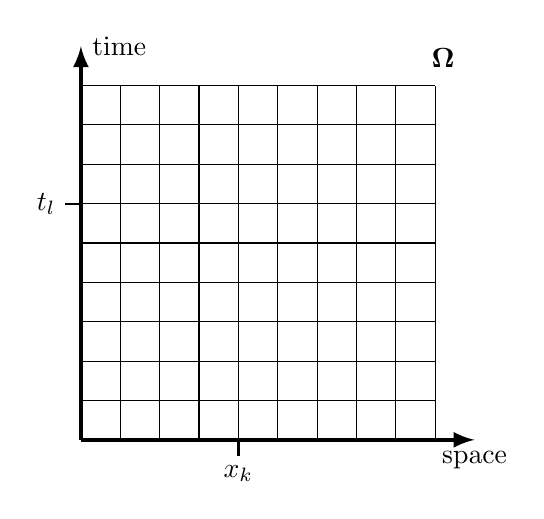
\begin{tikzpicture}
	% Draw the grid
	\tikzset{help lines/.style={color=black}}
	\draw[thin,step=0.5cm,help lines] (0,0) grid (4.5,4.5);
	
	% draw little line to indicate 
	\foreach \x in {2} {     % for x-axis
		\draw [thick] (\x,0) -- (\x,-0.2);
	}
	\foreach \y in {3} {   %% for y-axis
		\draw [thick] (0,\y) -- (-0.2,\y);
	}
	% draw label
	\foreach \x in {2} { \node [anchor=north] at (\x,-0.2) {$x_k$}; }
	\foreach \y in {3} { \node [anchor=east] at (-0.2,\y) {$t_l$}; }
	
	%\foreach \x in {0} { \node [anchor=north] at (\x,-0.2) {$(x_0, 0)$}; }
	\foreach \x in {4.6} { \node [anchor=north] at (\x,5.1) {$\mathbf{\Omega}$}; }
	
	% Draw axes
	\draw[ultra thick,-latex] (0,0) -- (5,0) node[below] {space};
	\draw[ultra thick,-latex] (0,0) -- (0,5) node[right]{time};
	% the co-ordinates -- major
	
	% the co-ordinates -- minor
	\end{tikzpicture}
	\label{fig:space_time_grid}
\end{figure}

which are defined by $N_x+1$ nodes in space and $N_t+1$ nodes in time. We will then refer to the tuples $(x_k, t_l)$ in the following manner, the $\tilde{i}$-th entry references $\tilde{i} = (N_x+1) \cdot l + k$. That is we first label all degrees of freedom belonging to a certain time step, such that $x_k < x_{k+1}$, before moving on to the next time step. 
\smallskip
\\
In our least-squares formulation we are dealing with the variables $\sigma$ and $u$, which are both defined on $\Omega$ and for which we have to construct an overall approximation space. However we have seen before that they can be defined indepedently and then combined later on. We chose to use the same individual approximation space as well as basis functions for both of them. This is possible because we are in the one-dimensional case and therefore $ \nabla u = \partial_x u = \sigma$ and $div(\sigma) = \partial_{x} \sigma$. For $dim (\mathcal{S}) > 1 $ we would have to treat this problem differently using for example Raviart-Thomas elements [source], which is beyond the scope of this thesis but would be of interest in future investigations. Therefore the following construction holds for each of them seperately and we will assemble the entire overall system later on. 
\smallskip
\\
As a finite-dimensional approximation space we used piecewise bilinear polynomials $Q_1(\Omega)$ in space--time. Given the reference element $\hat{K} = [0,1]^2$ we used the following basis on $\hat{K}$ \\

\begin{minipage}[l]{0.5\linewidth}

	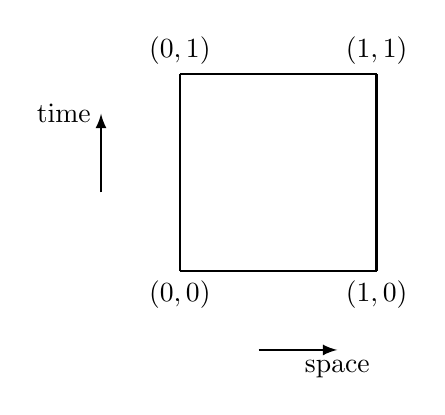
\begin{tikzpicture}
	% Draw the grid
	\tikzset{help lines/.style={color=black}}
	\draw[thick,step=2.5cm] (0,0) grid (2.5,2.5);
	

	 \node [anchor=north] at (0,0) {$(0,0)$};
	 \node [anchor=north] at (2.5,0) {$(1,0)$};
	 \node [anchor=south] at (0,2.5) {$(0,1)$};
	 \node [anchor=south] at (2.5,2.5) {$(1,1)$};
	 
	 
	 \draw[thick,-latex] (1,-1) -- (2,-1) node[below] {space};
	 \draw[thick,-latex] (-1,1) -- (-1,2) node[left]{time};
	 
	\end{tikzpicture}
\end{minipage}% 
\begin{minipage}[r]{0.5\linewidth}
\begin{ceqn}
	\begin{equation}
	\begin{aligned}
	\label{basis_function}
	\hat{\phi}_{11}(x,t) &= (1- x) &\cdot (1-t) \\
	\hat{\phi}_{12}(x,t) &=  x  &\cdot  (1-t) \\
	\hat{\phi}_{21}(x,t) &= (1- x) &\cdot t  \\
	\hat{\phi}_{22}(x,t) &= x  &\cdot  t 
	\end{aligned}
	\end{equation}
	\end{ceqn}
\end{minipage}
\textit{add caption to $\hat{K}$: reference element $\hat{K}$.} \\
Then the local space of the reference element is defined by $Q_1(\hat{K})$. There exist affine transformations $\{ \hat{P_{\zeta}}: \hat{K} \rightarrow K_{\zeta}\} $ to each of the mesh cells $K_{\zeta}$ which look as follows
\begin{ceqn}
	\begin{equation}
	\begin{aligned}
	\hat{P}_{\zeta} \begin{pmatrix}
	\hat{x} \\
	\hat{t}
	\end{pmatrix}= \begin{bmatrix}
	h_x & 0 \\
	0 & h_t
	\end{bmatrix}
	\begin{pmatrix}
	\hat{x} \\
	\hat{t}
	\end{pmatrix} + 	\begin{pmatrix}
	x_k \\
	t_l
	\end{pmatrix} , \quad \text{ for } (\hat{x}, \hat{t}) \in \hat{K}
	\end{aligned}
	\end{equation}
\end{ceqn}
if $K_{\zeta}$ is determined by the coordinates $\{(x_k, t_l), (x_{k+1}, t_k), (x_k, t_{l+1}), (x_{k+1}, t_{l+1})\}$. And which define the local spaces 

\begin{ceqn}
	\begin{equation}
	\begin{aligned}
Q_1(K_{\zeta}) = \{\phi : \phi = \hat{\phi} \circ \hat{P}_{\zeta}, \hat{\phi} \in Q_1(\hat{\phi})\}
	\end{aligned}
	\end{equation}
\end{ceqn}

\textit{global basis}
\begin{ceqn}
	\begin{equation}
	\begin{aligned}
	\phi_{ij}(x_k, t_l) = \begin{cases} 1 \quad \text{if } (k,l) = (i,j)  \\ 0 \quad \text{otherwise.} \end{cases} \quad (k, l) \in 
	\end{aligned}
	\end{equation}
\end{ceqn}

As previously mentioned $\sigma$ and $u$ are arranged such that they are two concatenated vectors. Hence one obtains a system of equations with $m = (N_x + 1 )\cdot (N_t + 1)$ degrees of freedom for $\sigma$ and $u$, respectively. The solution vector is therefore of size $2m$ while the matrices have a size of $2m \times 2m$. In order to compute the individual integral terms on the individual mesh cells we used Gaussian quadrature of order 3. The implemented admissible boundary conditions are a mixture of Dirichlet and Neumann type which get directly imposed in the system, respectively in either $u$ or $\sigma$. Hence we now have all the necessary ingredients to compute the individual terms arising from the discretisation in Chapter 4. 

\section{Multigrid Implementation}
We implemented a geometric multigrid V-cycle to solve the arising linear system of equations. It includes two different types of Vanka-smoothers which we will introduce below after discussing the coarse level construction.
 \textit{what else can I say here?}
\smallskip
\\
tried it with both Galerkin assembly and directly generating the operators on the coarse grid. lead to similar results. 

\subsection{Coarse Level Construction}
 An important question that always arises in every geometric multigrid implementation is how to choose the coarse level spaces. As discussed previously there is no unique optimal problem indepedent coarsening strategy, and especially in the case of space--time discretisations, the choice of the coarsening strategy has a great effect on the overall performance \cite{gander2016analysis}. There is not yet much literature on what could be a favourable strategy in a least-squares space--time set up and therefore we decided to use a classical space--time coarsening approach, for each $\sigma$ and $u$ independently. For each coarsening step the size of each rectangular element of in $\Omega$ grows by a factor of 4 with between each level while the length of the element doubles in each direction, see figure [...] below. It means that with each coarsening step the number of elements reduces by a factor of $(2^{-2})$ and hence the degrees of freedom accordingly.
 The paper of \cite{gander2016analysis} showed that space--time  multigrid implementations for second order parabolic equations it is favourable to keep the quotient $\lambda = D \frac{\Delta t}{\Delta x^2}$ (where $D$ decribes the diffusion constant and $\Delta t$ and $\Delta x$ the respective step sizes) close to one on all levels. However, as we are dealing with a mixed first order system here it seemed reasonable to not take this assumption into account but instead aim for $ \lambda = D \frac{\Delta t}{\Delta x} \approx 1$, which is in line with the coarsening strategy described above. In section (6.3.2) we will see some numerical test cases to investigate this assumption. %\textit{Rough estimates showed that for the linear case this seemed to be the case as a interpolation operators of type \cite{gander2016analysis} seemed to lead to slower convergence.} 
 The implementation is then such that one chooses the number elements on the coarse grid and the number of levels. And subsequently all other meshes, interpolation and restrictions operators, and finer level operators are generated automatically, according to the chosen paramaters, which guarantees for nested meshes.
\smallskip
\\
One still has to choose interpolation operators to project between levels, which we did according to the following scheme.  \\

\begin{minipage}[l]{0.5\linewidth}
	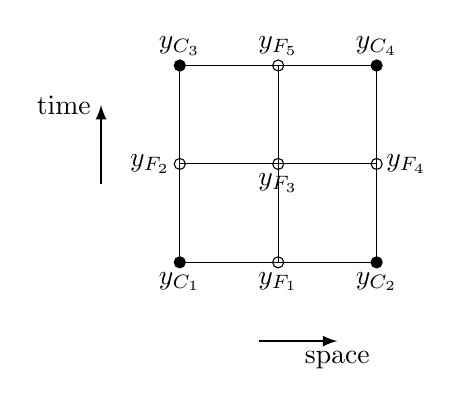
\begin{tikzpicture}
	% Draw the grid
	\tikzset{help lines/.style={color=black}}
	\draw[thin,step=1.25cm, help lines] (0,0) grid (2.5,2.5); 
	

    \draw[black, fill=black] (0,0) circle(2pt);
    \draw[black, fill=black] (2.5,0) circle(2pt);
    \draw[black, fill=black] (0,2.5) circle(2pt);
    \draw[black, fill=black] (2.5,2.5) circle(2pt);
    
    \draw[black] (1.25,0) circle(2pt);
    \draw[black] (0,1.25) circle(2pt);
    \draw[black] (1.25,1.25) circle(2pt);
    \draw[black] (2.5,1.25) circle(2pt);
    \draw[black] (1.25, 2.5) circle(2pt);
    
	 \draw[thick,-latex] (1,-1) -- (2,-1) node[below] {space};
	\draw[thick,-latex] (-1,1) -- (-1,2) node[left]{time};
	
	\node [anchor=north] at (0,0) {$y_{\text{C}_1}$};
	\node [anchor=north] at (2.5,0) {$y_{\text{C}_2}$};
	\node [anchor=south] at (0,2.5) {$y_{\text{C}_3}$};
	\node [anchor=south] at (2.5,2.5) {$y_{\text{C}_4}$};
	
	\node [anchor=north] at (1.25,0) {$y_{\text{F}_1}$};
	\node [anchor=east] at (0,1.25) {$y_{\text{F}_2}$};
	\node [anchor=north] at (1.25,1.25) {$y_{\text{F}_3}$};
	\node [anchor=west] at (2.5,1.25)  {$y_{\text{F}_4}$};
	\node [anchor=south] at (1.25,2.5) {$y_{\text{F}_5}$};
	
	\end{tikzpicture}
	\textit{add caption. filled circles represent coarse grid points and the blank circles fine grid points. $y$ stands for the values at each of the nodes.}

\end{minipage}%
\begin{minipage}[r]{0.5\linewidth}
\begin{ceqn}
	\begin{equation}
	\begin{aligned}
	s(y_{\text{C}_i})  &= s(y_{\text{C}_i})  \qquad \forall i \\	
	s(y_{\text{F}_1}) &= \frac{1}{2} y_{\text{C}_1} + \frac{1}{2} y_{\text{C}_2} \\
	s(y_{\text{F}_2}) &= \frac{1}{2} y_{\text{C}_1} + \frac{1}{2} y_{\text{C}_3} \\
	s(y_{\text{F}_3}) &= \frac{1}{4} y_{\text{C}_1} + \frac{1}{4} y_{\text{C}_2} + \frac{1}{4} y_{\text{C}_3} + \frac{1}{4} y_{\text{C}_4} \\		
	s(y_{\text{F}_4}) &= \frac{1}{2} y_{\text{C}_2} + \frac{1}{2} y_{\text{C}_4} \\
	s(y_{\text{F}_5}) &= \frac{1}{2} y_{\text{C}_3} + \frac{1}{2} y_{\text{C}_4} \\
	\end{aligned}
	\end{equation}
	\end{ceqn}
\\
\end{minipage}
If $\tilde{I}$ is an interpolation operator of the above type is defined between two levels then they can be applied for either $\sigma$ or $u$. Hence in order to obtain an interpolation for both we assemble them in the following form 
\begin{ceqn}
	\begin{equation}
	I = \begin{bmatrix}
	\tilde{I} & 0 \\
	0 & 	\tilde{I}
	\end{bmatrix}
	\end{equation}
\end{ceqn}
That is the two variables are interpolated indepedently, which seems reasonable, since on the one hand they are clearly related but as one is the spatial derivative of the other, this is difficult to express in an interpolation operator. The arising matrix from level $k-1$ to level $k$ is as before denoted by $I_{k-1}^k$ and we have that  $I_{k-1}^k \in \mathbb{R}^{2m_k \times 2m_{k-1}}$, where $m_k$ and $m_{k-1}$ denotes the number of points on the space time grid on the respective level. Below we can see example of the application of an interpolation operator above type $\tilde{I}$.

\begin{figure}[ht!]
	\centering
	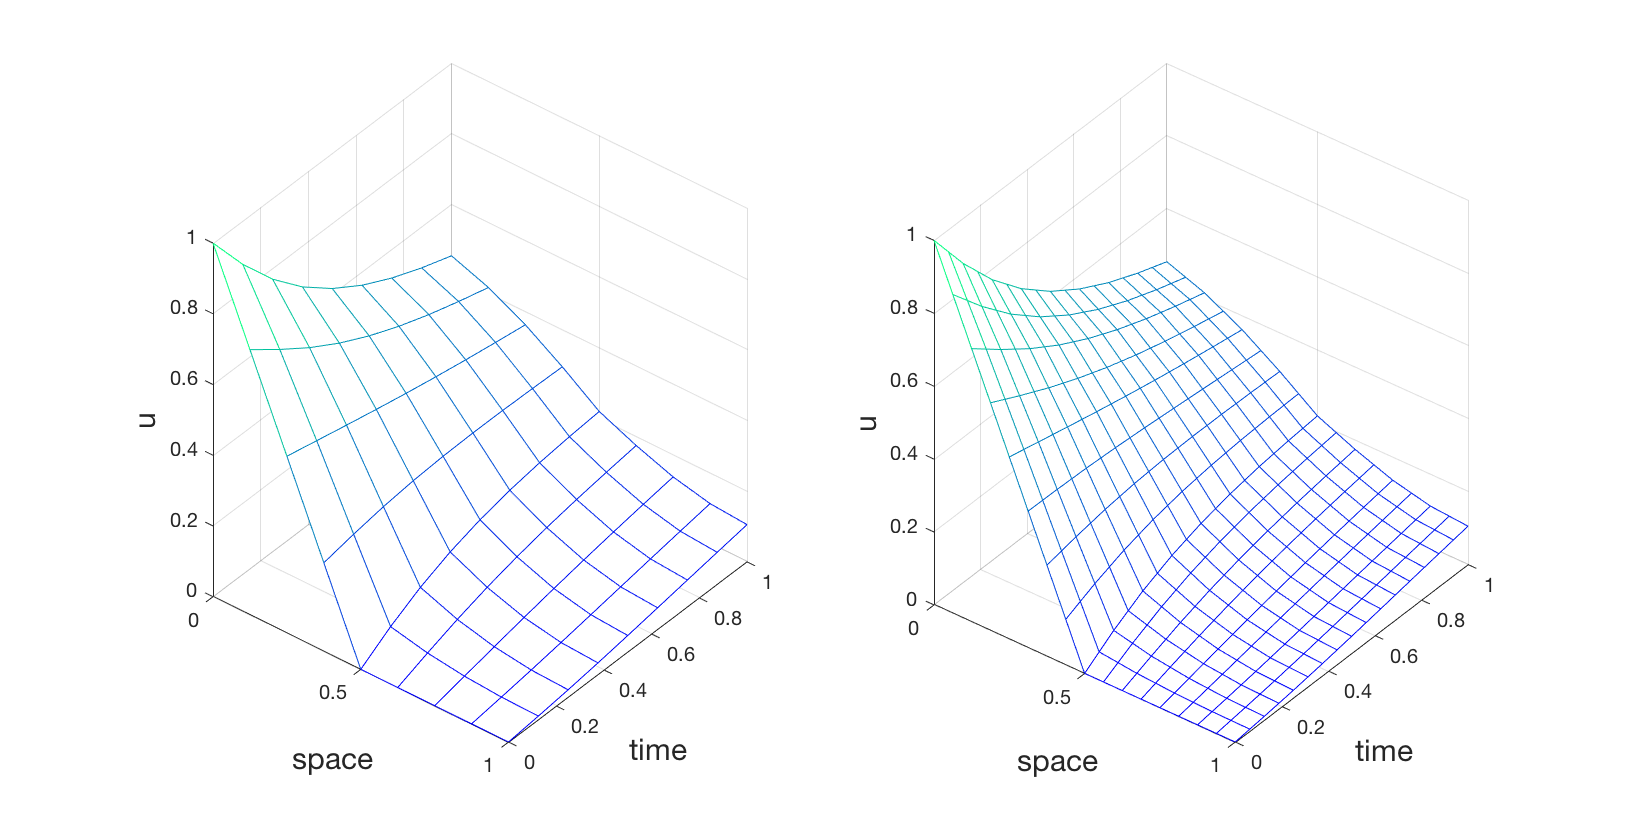
\includegraphics[scale=0.25]{images/implementation/sol_heat_eqn_interpol}
	\caption{Interpolation of the solution to the heat equation with $u(x,0) = \max(1-2x, 0)$, $D(x) = 0.1$ and homogeneous Neumann boundary conditions in time on a unit square from $8 \times 8$ to $16 \times 16$ elements. The interpolated solution of $\sigma$ is not shown here as $\tilde{I}$ simply applied to $\sigma$ and $u$ independently.}
	\label{fig:interpolation_op}
\end{figure}

\textbf{Remark:} In the implemenation of the multigrid V--cycle we remove the influence of the boundary conditions as in linear multigrid we apply the coarse grid correction on the error and therefore cannot have a correction coming from a fixed boundary. 

\FloatBarrier
\subsection{Smoothers}
Smoothers are a key part of a multigrid algorithm. We would like that the combination of coarse grid correction and smoother reduces the error efficiently. But as this is a complicated interplay of two processes it is often not easy to determine in advance what would be a suitable choice for a smoother. In the case of a geometric multigrid applied to an elliptic problem the coarse grid correction captures the low frequency error quickly while most smoothers like (block-) Jacobi or Gauss-Seidel reduce the high frequency error well and therefore the either of the two combined with the coarse grid correction are a favourable synthesis. Since we are also trying to develop a parallelisable solver it is of course important to also be taking that into account when choosing a smoother. Thus a regular Gauss-Seidel iteration is for example not a suitable choice, as it works sequentially. In our set up we also have the additional feature of the two coupled variables $\sigma_h$ and $u_h$, which are separated in the matrix-vector assembly as two concatenated vectors but have the contentual connection. Therefore it might be favorable to use a (block-) smoother that takes this relationship into account. Hence we decided to use a Vanka type [source?] damped block Jacobi relaxation. That is a damped block Jacobi smoother where each block contains all degrees of freedom associated to one grid point in the space--time domain. One can choose $p$ degrees of freedom in space and $q$ in time, to obtain a rectangular patch with $p \times q$ degrees of freedom on the domain. Then the algorithm constructs a submatrix containing all entries of $A$ associated to those nodes for $\sigma$ and $u$ as well as all of the corresponding coupling terms and directly inverts the small submatrix. The entire domain is partitioned in this way. On the boundary we might potentially obtain smaller patches, depending on the divisibility of the chosen patch size. In this way we obtain a preconditioner $P$ containing the inverted submatrices. Due to the organisation of $\sigma$ and $u$, $P$ will not be a block diagonal matrix. For $p = q = 2 $ we would have the following patches, where $\tilde{c}_i$ describes the set of indices assosciated with the patch, and $C_i$ the corresponding submatrix, which are each of size $8 \times 8$. 

\begin{figure}[ht!]
	\centering
	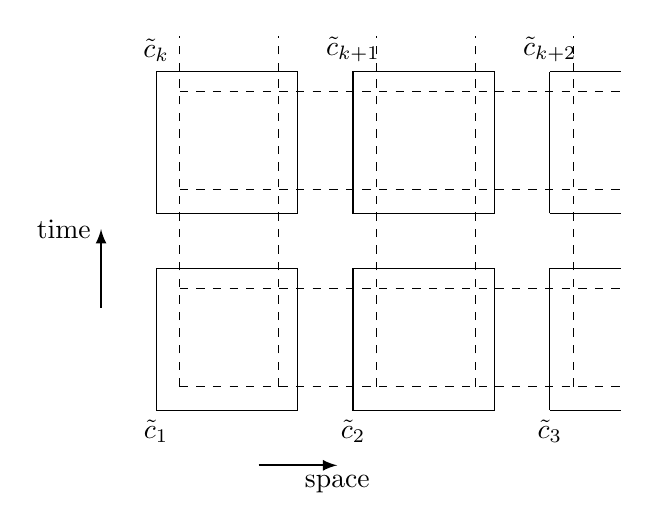
\begin{tikzpicture}
	% Draw the grid
	\tikzset{help lines/.style={color=black, dashed}}
	\draw[thin,step=1.25cm, help lines] (0,0) grid (5.6,4.45); 
	
	\draw[thick,-latex] (1,-1) -- (2,-1) node[below] {space};
	\draw[thick,-latex] (-1,1) -- (-1,2) node[left]{time};
	
	\draw[black] (-0.3,-0.3) rectangle  (1.5,1.5);
	\draw[black] (2.2,-0.3) rectangle  (4,1.5);
	
	\draw[black] (-0.3,2.2) rectangle  (1.5,4);
	\draw[black] (2.2,2.2) rectangle  (4,4);
	
	\draw[black] (4.7, -0.3) -- (5.6,-0.3);
	\draw[black] (4.7, -0.3) -- (4.7, 1.5);
	\draw[black] (4.7, 1.5) -- (5.6,1.5);	
	
	\draw[black] (4.7, 2.2) -- (5.6,2.2);
	\draw[black] (4.7, 2.2) -- (4.7, 4);
	\draw[black] (4.7, 4) -- (5.6,4);	
	
	\node [anchor=north] at (-0.3,-0.3) {$\tilde{c}_1$};
	\node [anchor=north] at (2.2, -0.3) {$\tilde{c}_2$};
	\node [anchor=north] at (4.7, -0.3) {$\tilde{c}_3$};	
	
	\node [anchor=south] at (-0.3,4) {$\tilde{c}_k$};
	\node [anchor=south] at (2.2, 4) {$\tilde{c}_{k+1}$};
	\node [anchor=south] at (4.7, 4) {$\tilde{c}_{k+2}$};		
	\end{tikzpicture}
	\caption{Schematic overview of the construction of the blocks of damped Jacobi smoother}
\end{figure}

Below we can see how the smoother acts on a random initial guess for the linear system $As = f$, where $A$ is the least squares finite element matrix arising from the functional $J([\sigma, u], 0)$ with the discretisation chosen as described in chapter 4 and the previous parts of this chapter, and $f$ is a zero right-hand side that only contains the boundary conditions. That is we look at the iteration 
\begin{ceqn}
	\begin{equation}
	e_{k+1} = e_k + \omega P (f - Ae_k)
	\end{equation}
\end{ceqn}
where $P$ is the preconditioner and $\omega$ stands for the damping factor. Since we have a zero forcing term, the exact solution is zero everywhere if we have homogenous boundary conditions, and hence $e_k$ describes the remaining error in each iteration starting from an initial guess. 

% for contourplot 1 it took 8184 iterations to have residual <10^(-9)

\begin{figure}[ht!]
	\centering
	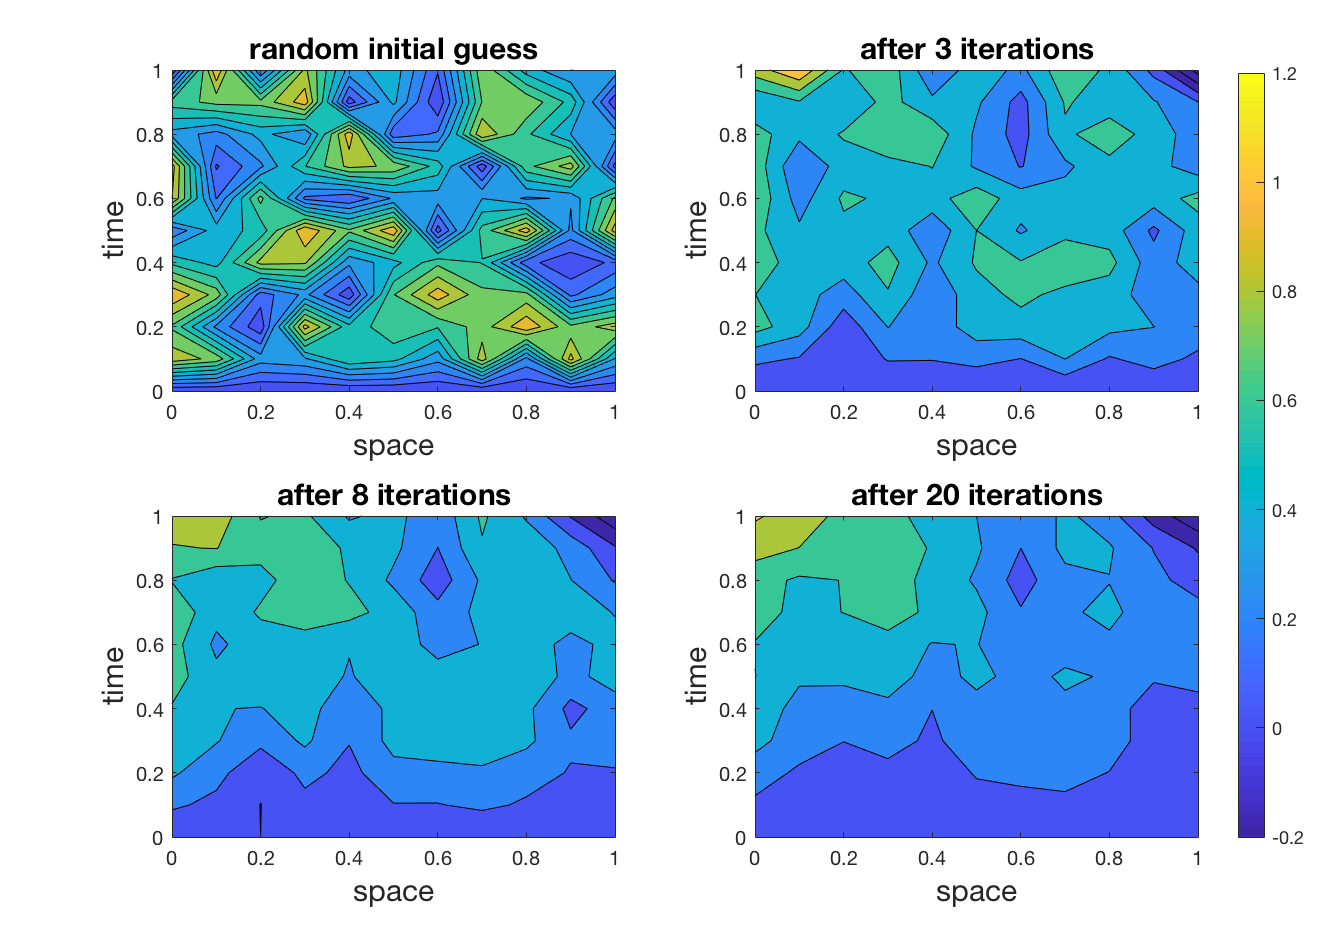
\includegraphics[width=0.9\textwidth]{images/implementation/contour_plot_1_blk_size1by1}
	\caption{Iterates after $k = 0,3,8, 20$ iterations for a patch size of $1 \times 1$, and a grid with $11 \times 11$ elements. needed more than 9000 iterations in order for the norm of the residual to be smaller than $ 10^{-9}$. }
	\label{fig:smoother_1by1}
\end{figure}

We can see that the damped block Jacobi smoother really leads to a fast reduction of the high frequency error whereas the low frequency error is only reduced very slowly. We again only plotted the results for $u$ as $\sigma$ behaves in the same way, simply with different boundary conditions. We also compared the performance of the this smoother for different block sizes. As one would expect it reduces the error faster for larger block sizes. We can see that by comparing the number of overall iterations until the stopping criterion was met as well as by looking at the graphs which show less oscillations for the larger patch as well as values closer to zero. The damping factor was $\omega = \frac{2}{3}$ in both cases.  
\smallskip
\\
\begin{figure}[ht!]
	\centering
	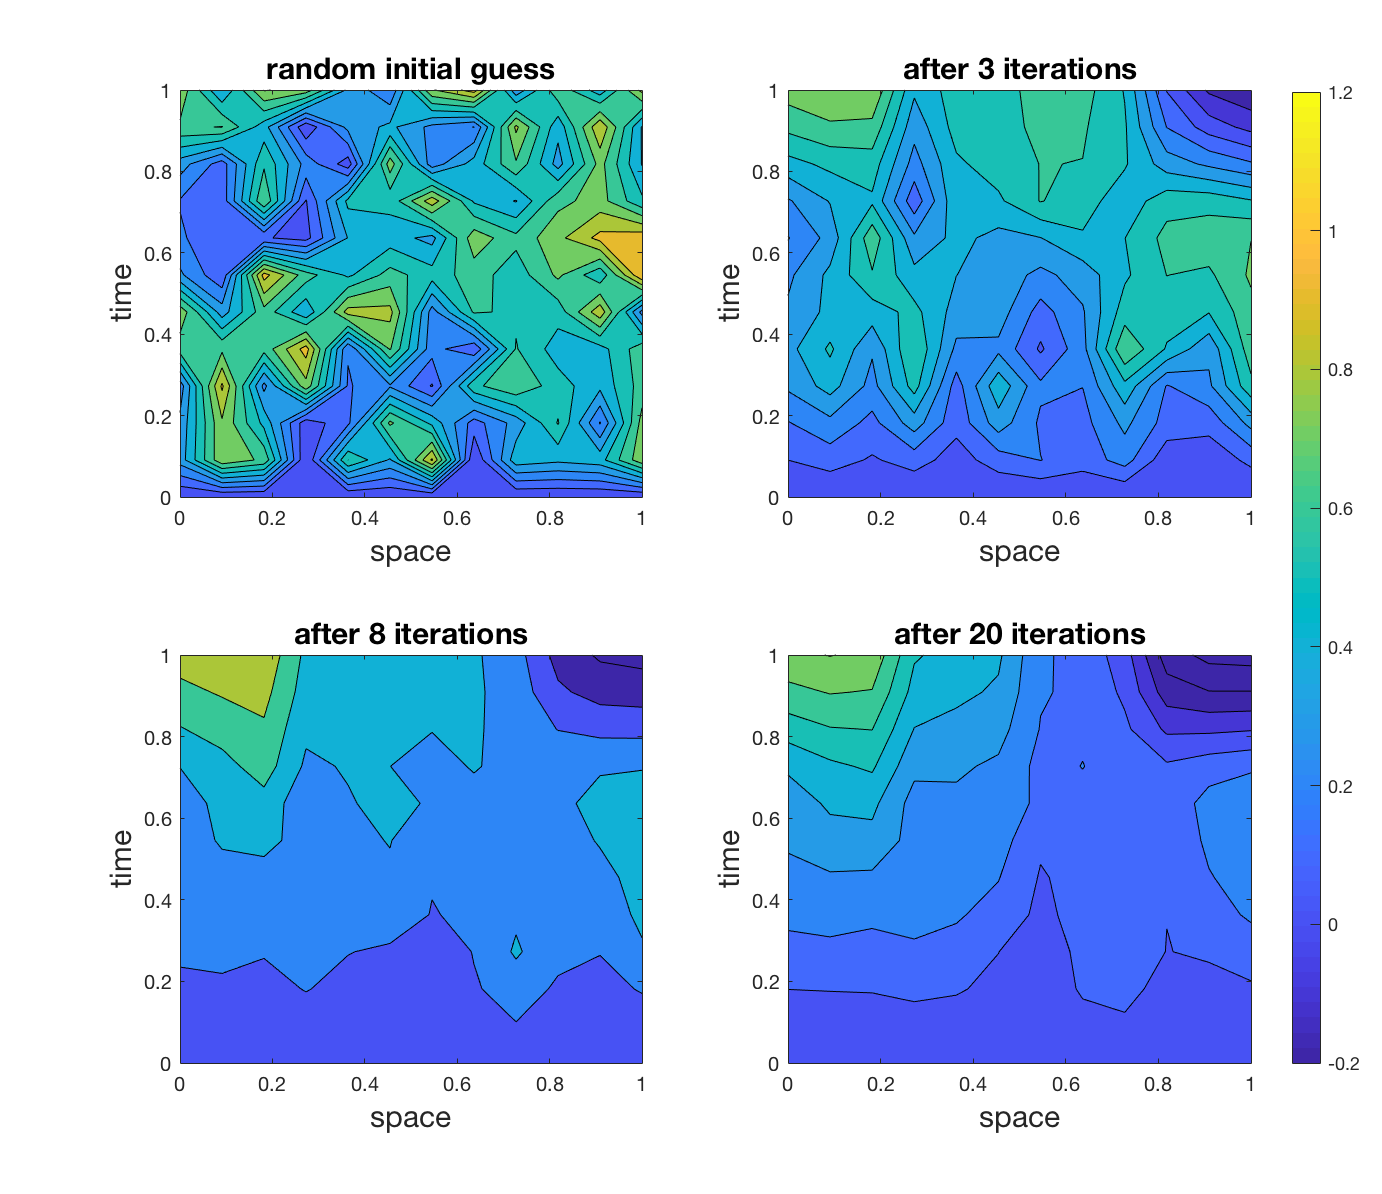
\includegraphics[width=0.9\textwidth]{images/implementation/contour_plot_1_blk_size3by4}
	\caption{Iterates after $k = 0,3,8, 20$ iterations for a patch size of $3 \times 4$, and a grid with $11 \times 11$ elements. needed more than 3177 iterations in order for the norm of the residual to be smaller than $ 10^{-9}$.}
	\label{fig:smoother_3by4}
\end{figure}

Another type of smoother that we tested is a Gauss-Seidel line smoother which is similar to works of \cite{adams2001distributed} and can also be categorised as a Vanka smoother. One considers each spatial degree of freedom individually but together for all times as well as the values for $\sigma$ and $u$. We extract all matrix values for each of the $x_i$, to construct submatrices. We then first solve exactly for all odd subsets of $\tilde{c}_i$, here coloured in black and update the solution before solving for all even subsets, here coloured in red. Hence for all subsets labeled in black we can solve in parallel, and subsequently for all subsets in red. 

\begin{figure}[ht!]
	\centering
	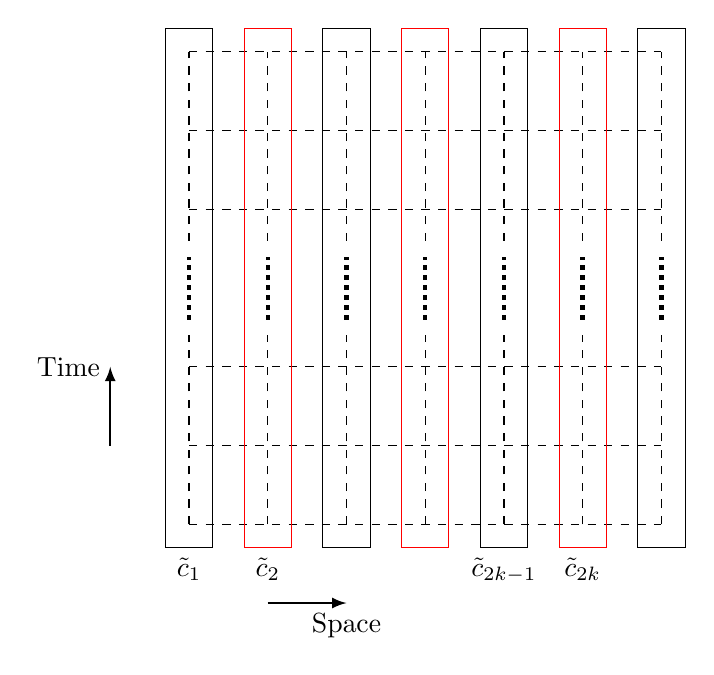
\begin{tikzpicture}
	% Draw the grid
	\tikzset{help lines/.style={color=black, dashed}}
	\draw[thin,step=1cm, help lines] (0,0) grid (6,2.4); 	
	\draw[thin,step=1cm, help lines] (0,3.6) grid (6,6); 
	
	\draw [black, dotted, ultra thick] (0, 2.6) -- (0, 3.4);
	\draw [black, dotted, ultra thick] (1, 2.6) -- (1, 3.4);
	\draw [black, dotted, ultra thick] (2, 2.6) -- (2, 3.4);
	 \draw [black, dotted, ultra thick] (3, 2.6) -- (3, 3.4);
	 \draw [black, dotted, ultra thick] (4, 2.6) -- (4, 3.4);
	\draw [black, dotted, ultra thick] (5, 2.6) -- (5, 3.4);
	\draw [black, dotted, ultra thick] (6, 2.6) -- (6, 3.4);		  
		  
	\draw[thick,-latex] (1,-1) -- (2,-1) node[below] {Space};
	\draw[thick,-latex] (-1,1) -- (-1,2) node[left]{Time};
	
	\draw[black] (-0.3,-0.3) rectangle  (0.3,6.3);
	\draw[red] (0.7,-0.3) rectangle  (1.3,6.3);
	\draw[black] (1.7,-0.3) rectangle  (2.3,6.3);
	\draw[red] (2.7,-0.3) rectangle  (3.3,6.3);
	\draw[black] (3.7,-0.3) rectangle  (4.3,6.3);
	\draw[red] (4.7,-0.3) rectangle  (5.3,6.3);
	\draw[black] (5.7,-0.3) rectangle  (6.3,6.3);	
	
	\node [anchor=north] at (0,-0.3) {$\tilde{c}_1$};
	\node [anchor=north] at (1, -0.3) {$\tilde{c}_2$};
	
	\node [anchor=north] at (4, -0.3) {$\tilde{c}_{2k-1}$};	
	\node [anchor=north] at (5, -0.3) {$\tilde{c}_{2k}$};					
	
	\end{tikzpicture}
	\caption{Schematic overview of the construction blocks in the Gauss Seidel line smoother}
\end{figure}

We repeated the same test as before where the preconditioner $P$ is now defined by the above description. 

\begin{figure}[ht!]
	\centering
	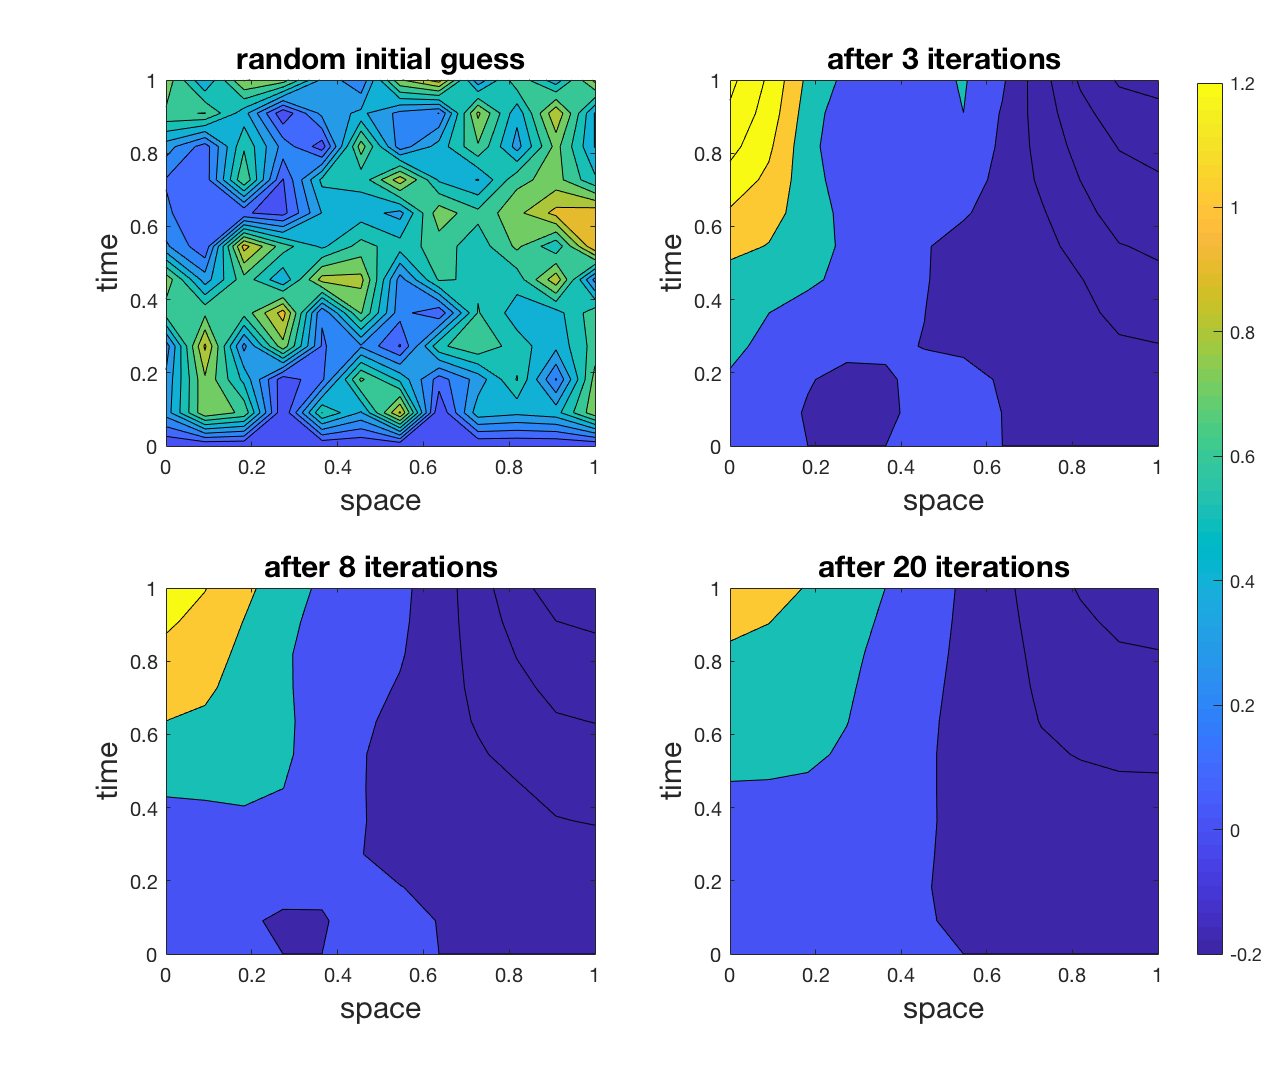
\includegraphics[scale=0.28]{images/implementation/contour_plot_1_lineSm}
	\caption{Iterates after $k = 0,3,8, 20$ iterations for the described line smoother, using a grid with $11 \times 11$ elements. It needed more than about 1759 iterations in order for the norm of the residual to be $< 10^{-9}$. where $A, f$ as before}
\end{figure}

As one might expect the line smoother converges much faster than the block Jacobi iteration, since the individual blocks we solve for exactly are larger. We can also see that the regions become more homogenous more quickly. \textit{there are quite large areas where we go below 0, why?}. But obviously this comes with an increase in the computational cost. 
\\
Performs much better than 3 by 4, why? Gauss Seidel? 

\FloatBarrier
\section{Numerical Test Cases}

\subsection{One-Dimensional Poisson Equation}
\label{ssec:Poisson}

After having discussed the individual multigrid terms let us look at the overall multigrid performance. As a very first test case we construct a one-dimensional Poisson problem using the least squares set up. Of course this problem could be solved more easily using for example a primal weak formulation however this can serve us as a an simple test case for the multigrid implementation. We would like to remark here, that it necessarily has to be a one-dimensional problem in space, as we would otherwise have to use a different set of basis functions, like Raviart-Thomas basis functions, to obtain a well-defined discretisation, which would then not be using later on. Hence we want to find an approximate solution to the continuous minimisation problem

\begin{ceqn}
	\begin{equation}
	\begin{aligned}
	\text{Find } [\sigma, u] \in H_{\di}(\mathcal{S}) \times H^1(\mathcal{S}) \text{ such that } \hat{J}([\sigma, u], f) \text{ is minimal, with } \\
\hat{J}([\sigma, u], f) = \frac{1}{2}|| - div(\sigma) - f ||_{L^2(\mathcal{S})}^2  + \frac{1}{2} || \sigma - \nabla u ||_{L^2(\mathcal{S})}^2.
	\end{aligned}
	\end{equation}
\end{ceqn}
where we assume $f = f(x,t)$ and use the multigrid algorithm described above to solve the arising linear system of equations, only adapting the interpolation and restriction operators to suit a one-dimensional problem, standard one used here, see e.g. \cite{briggs2000multigrid} for details.

\begin{table}
	\begin{center}
		\begin{tabular}{||c | c | c | c ||} 
			\hline
			test case & degrees of freedom & iter until conv & avg conv rate \\ [0.5ex] 
			\hline\hline
			1 & 200 & 9 &  $3.81 \cdot 10^{-2}$ \\ 
			\hline		
			2 & 500 & 9 & $3.82 \cdot 10^{-2}$ \\ 
			\hline
			3 & 2000 & 10 &   $4.59 \cdot 10^{-2}$   \\
			\hline
			4 & 5000 & 10 &  $5.03 \cdot 10^{-2}$ \\
			\hline
		\end{tabular}
	\end{center}
	\caption{tall test cases on $\mathcal{S} = (0,3)$, with $u(0) = 3$, $u(1) = 0$, initial iterate $u_{\text{init}} = 1$, $\sigma_{\text{init}} = 0.5$, $f = 0$ and only vary in the number of degrees of freedom, that is the resolution of the mesh. Smoother: Jacobi-smoother, patch size $1 \times 1$. Convergence criterium : norm of residual smaller than $10^{-9}$.}
	\label{table:Table_mg_poisson}
\end{table}

The number of elements was chosen to roughly match the number of elements we will consider in the following sections to make the results more comparable, however as we only coarsen in space here. The iterations until convergence counts the number of $V$-cycles needed to read a residual norm smaller than $10^{-9}$ using 3 pre-and post smoothing steps, using a 2 levels. The local convergence rate is defined as $\mu_k = \frac{res_k}{res_{k-1}}$, where $k$ stands for the current iterate, and the overall convergence rate $\mu$ is defined as its geometric mean over all iterations. Hence the smaller the value is, that is the closer to zero the better is the update. If we have $\mu_k > 1$, it means that the residual actually increased from one iteration to another. The first values of $\mu_k$ highly depend on the initial guess but we can see below that later on that the average value is around $0.05$ which is of course a very fast rate of convergence, however our test case is also very simple, so one would also expect the algorithm to converge very quickly.

\begin{figure}[h!]
	\centering
	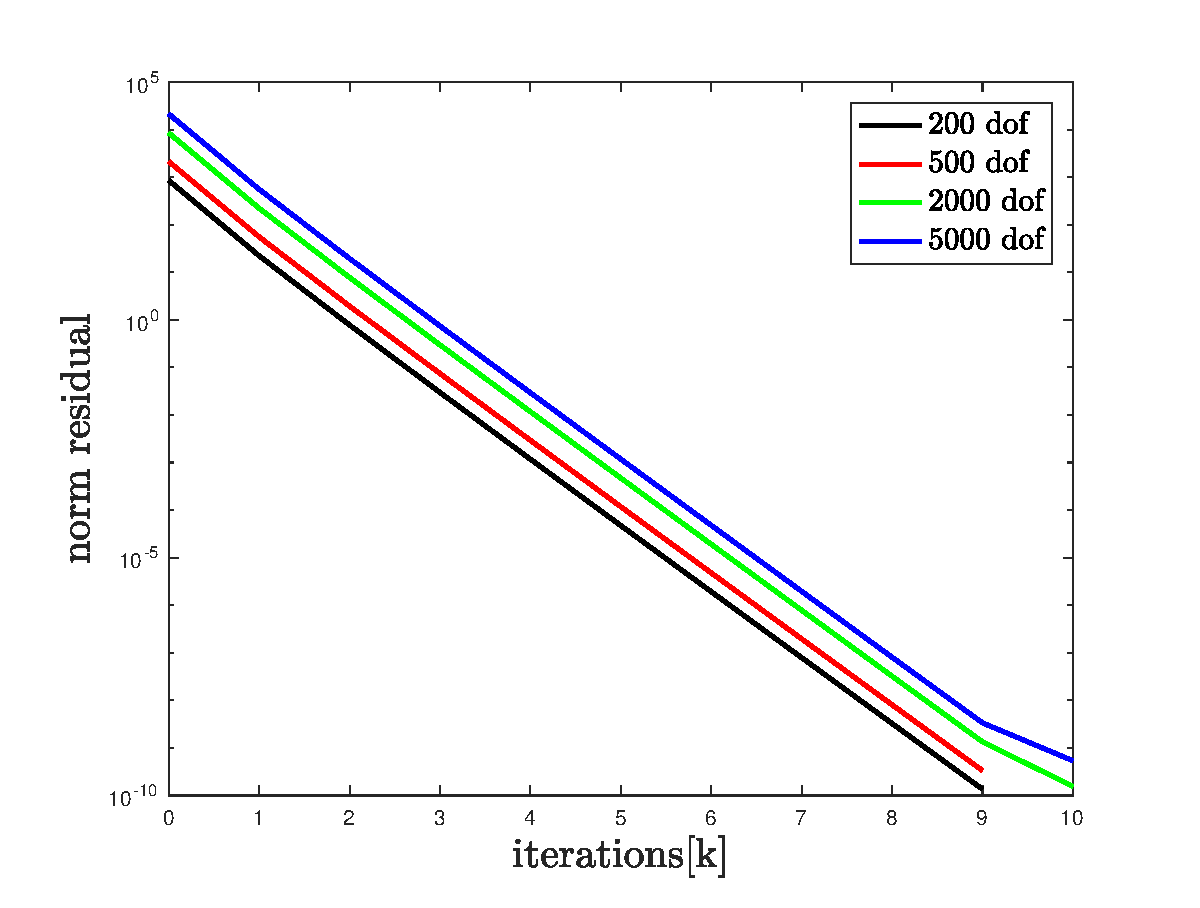
\includegraphics[width=0.45\textwidth]{images/implementation/poisson/residual_norm_mg}
	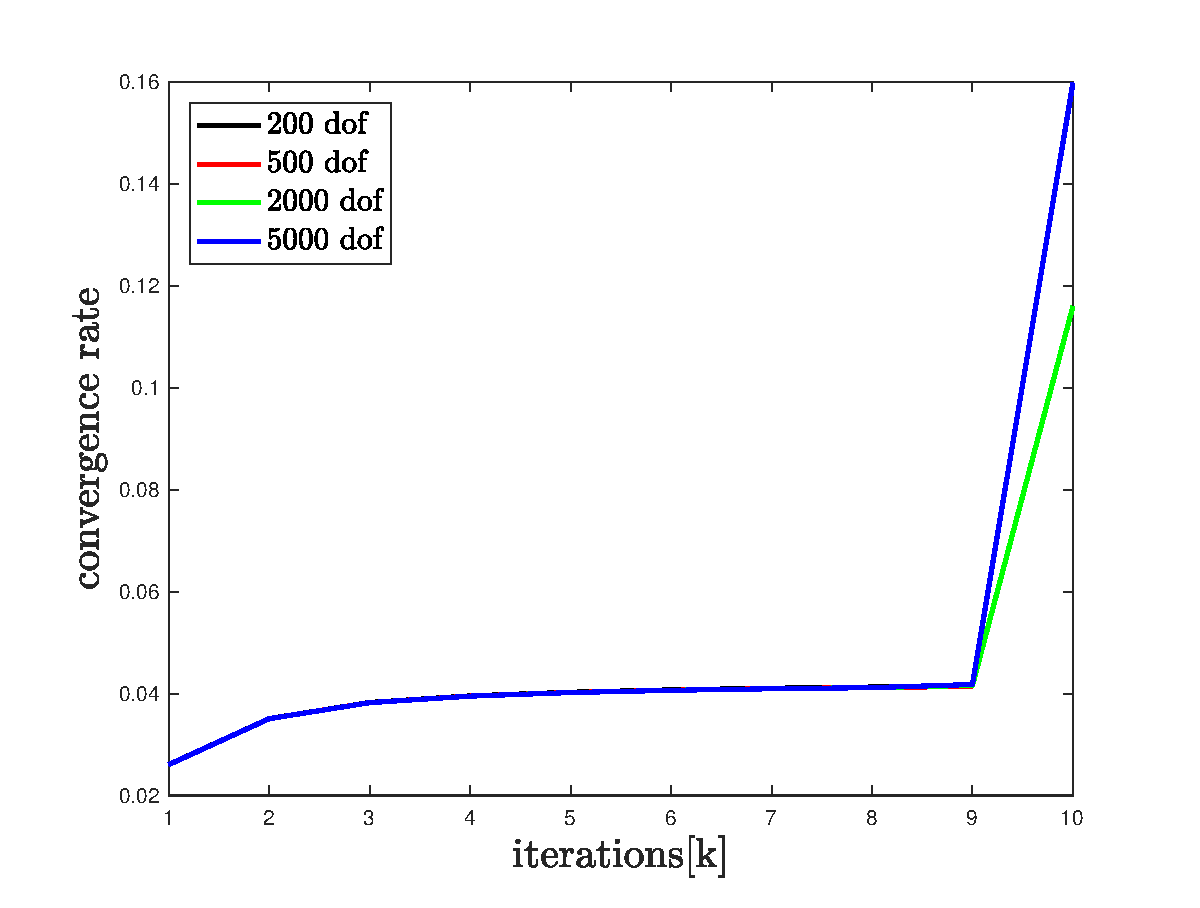
\includegraphics[width=0.45\textwidth]{images/implementation/poisson/convergence_rate_mg}
	\caption{Left-Panel: norm of the residual over iterations for test cases 1 to 4, Right-Panel: Convergence rate $\mu$ for test cases 1 to 4. See Table (\ref{table:Table_mg_poisson}) for details.}
	
\end{figure}
The pictures of the overall solution are not provided here, but they match the expected solutions in all test cases. Hence we can conclude that for these simple test cases the set up of the least squares formulation as well as the multigrid implementation work \textit{reasonably} well.

\FloatBarrier
\subsection{Heat Equation}

In this section we tested the multigrid implementation on our least-squares space--time finite element formulation imposing a zero forcing term. The continuous form of the functional which we want to minimise is shown here again

\begin{ceqn}
	\begin{equation}
	\begin{aligned}
	\label{J_heat_equation}
	J([\sigma, u], 0) = \frac{1}{2} c_1 || u_t - div(\sigma) ||_{L^2(\Omega)}^2 + \frac{1}{2} c_2 || \sigma - D \nabla u ||_{L^2(\Omega)}^2.
	\end{aligned}
	\end{equation}
\end{ceqn}

The multigrid algorithm converged for all tested input parameters. However there seem to be a lot different factors influencing the speed of convergence. The figure below shows the norm of the residual over the number of iterations for different numbers of degrees of freedom. 

\begin{figure}[h!]
	\centering
	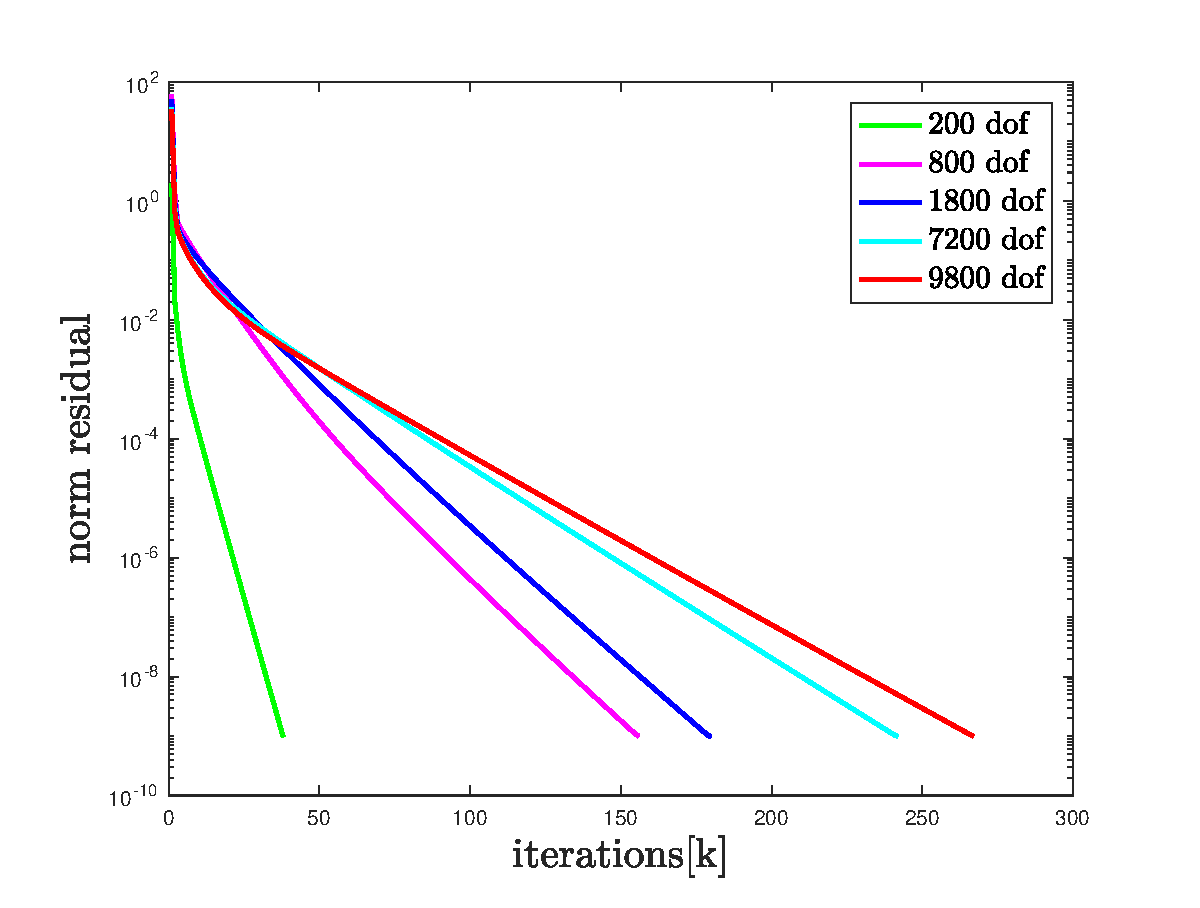
\includegraphics[scale=0.4]{images/implementation/multigrid_scaling/norm_res_scaling_mg}
		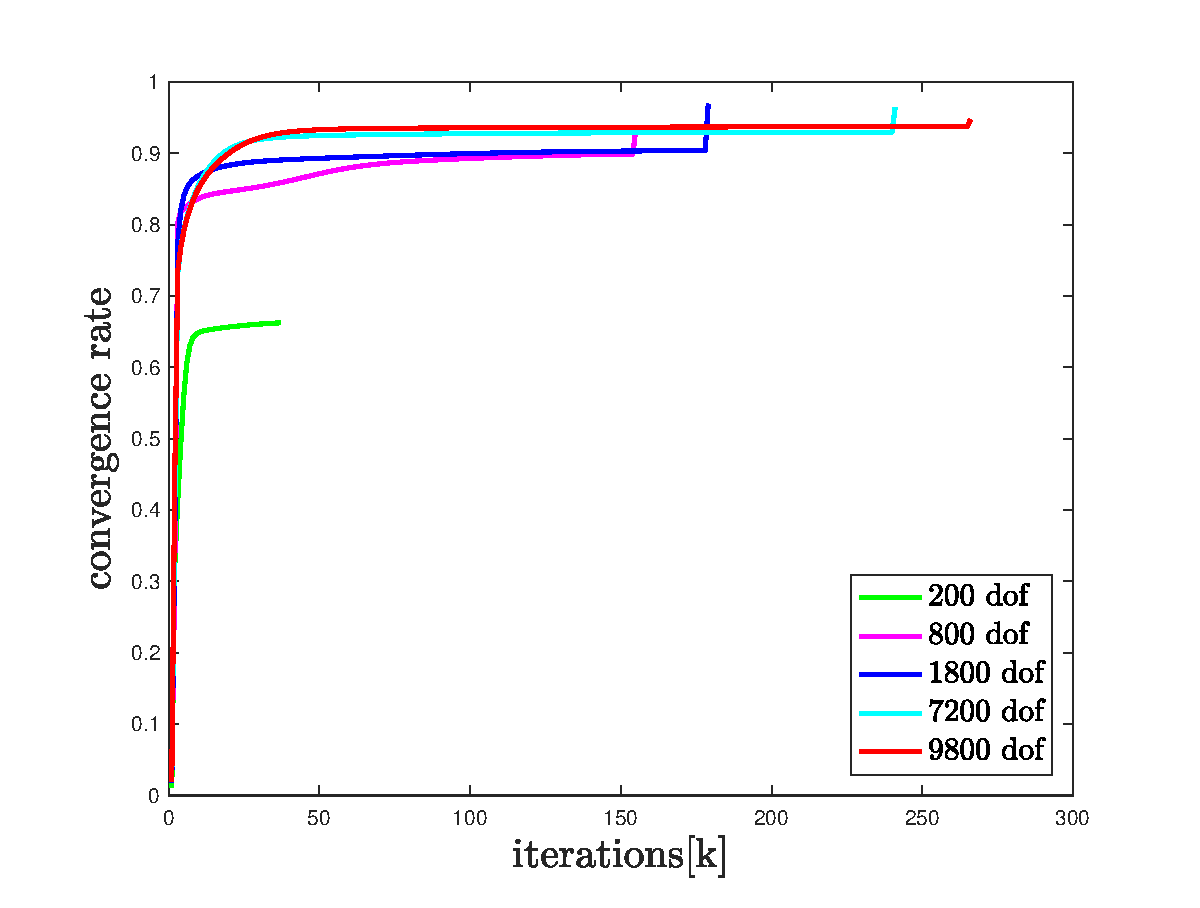
\includegraphics[scale=0.4]{images/implementation/multigrid_scaling/convergence_rate_scaling_mg}
	\caption{Left-Panel: Norm of the residual over iterations. Right-Panel: Convergence rate $\mu$. Stopping criterion residual norm smaller than $10^{-9}$, $\Omega = (0,1)^2$, same number of elements in time and space, $d = 1$, $c_2 = 100$, 2 level methods, 3 pre --and post smoothing steps, block Jacobi, patch size $2 \times 2$.}
	\label{fig:scaling_mg}
\end{figure}

In general it also seems that the required number of iterations until we reach the stopping criterion is quite large even though the tested problems are still very small. \textit{Problem sort of scales but not great. more later.} In order to find out what might be the cause, we varied different input parameters to see how it would affect the convergence results. The ones we want to mainly focus on are grid size and grid size ratio, a varying diffusion constant, and the interplay of the scaling factors of $c_1$ and $c_2$. We can find a table below that lists different parameters properties as well as the corresponding convergence results, like the number of required V-cycle and the convergence rate. This is meant to give an overview of the behavior of this solution method. Subsequently we will go into more detail concerning the affects of the individual input parameters to gain a better understanding for each of them. 

% add column with number of elements?!
\begin{table}[]
	\centering
	\begin{tabular}{||c|c|c|c|c|c|c|c||}
		\toprule
		sample & $N_x$ & $N_t$ & $d$ & $c_2$ & Iter until Conv & $\mu$ & $\kappa(H)$  \\
		\bottomrule
		\toprule
		1 & 10 & 10 & 0.1 & 1 & 98 & 0.858 & 1251 \\ \hline
		2 & 20 & 20 & 0.1 & 1 & 205 & 0.900 & 4707 \\ \hline
		3 & 30 & 30 & 0.1 &  1 & 403 & 0.947 & 10296 \\ 
		\toprule
		4 & 10 & 10 & 1 & 1 & 91 & 0.790 & 312 \\ \hline
		5 & 20 & 20 & 1 & 1 & 313 & 0.933 & 1505 \\ \hline
		6 & 30 & 30 & 1 & 1 & 641 & 0.966 & 3675 \\ 
		\toprule
		7 & 10 & 10 & 0.01 & 1 & 375 & 0.945 & 3561 \\ \hline
		8 & 20 & 20 & 0.01 & 1 & $\approx 800$ & $\approx 0.973$ & 19735 \\ \hline
		9 & 30 & 30 & 0.01 & 1 & $>800$ & $>0.981$ & 55902 \\ 
		\bottomrule
		\toprule
		10 & 10 & 10 & 0.1 & 10 & 36 & 0.551 & 214 \\ \hline
		11 & 20 & 20 & 0.1 & 10 &  91 & 0.788 & 765 \\ \hline
	    12 & 30 & 30 & 0.1 &  10  & 213 & 0.902 & 1651 \\ 
		\toprule
		13 & 10 & 10 & 1 & 10 & 40 & 0.563 & 1902 \\ \hline
		14 & 20 & 20 & 1 & 10 & 116 & 0.822 & 7090 \\ \hline
		15 & 30 & 30 & 1 & 10 & 236 & 0.909 & 15521 \\ 
		\toprule
		16 & 10 & 10 & 0.01 & 10 &   274 & 0.925 & 1084 \\ \hline
		17 & 20 & 20 & 0.01 & 10 &  413 & 0.949 & 4115 \\ \hline
		18 & 30 & 30 & 0.01 & 10 & 740 & 0.971 & 8977 \\ 
		\bottomrule
	     \toprule
		19 & 10 & 10 & 0.1 & 100 & 12 & 0.163 & 215 \\ \hline
		20 & 20 & 20 & 0.1 & 100 & 25  & 0.418 & 732 \\ \hline
		21 & 30 & 30 & 0.1 &  100 &  49 & 0.638 & 1574 \\ 
		\toprule
		22 & 10 & 10 & 1 & 100 & 169 & 0.862 & 19006 \\ \hline
		23 & 20 & 20 & 1 & 100  & 155 & 0.852 & 70890\\ \hline
		24 & 30 & 30 & 1 & 100 &  179 & 0.871 & 155190 \\ 
		\toprule
		25 & 10 & 10 & 0.01 & 100 & 81 & 0.768 & 322 \\ \hline
		26 & 20 & 20 & 0.01 & 100 & 84 & 0.772 & 895 \\ \hline
		27 & 30 & 30 & 0.01 & 100 & 112 & 0.822 &  1792\\ 
		\bottomrule
	\end{tabular}
\caption{Overview of a number of sample cases, tested for varying parameters in the number of fine elements $N_x$, the number of fine elements in time $N_t$, the diffusion constant $D$ and the scaling parameter $c_2$. The iterations until convergence give the number of V-cycles, using a 2-level method with 3 pre-and post smoothing steps of the block Jacobi smoother introduced before, with a patch size of $2 \times 2$, and $\kappa(H)$ denotes the condition number of the symmetrised Hessian}
	\label{table:convergence_results}
\end{table}

We can see that number of iterations needed until the convergence criterion is met differs greatly. Changes in some paramters seem to have a straight forward correlation with the convergence speed while with others this does not appear to be the case. So let us discuss them in more detail one by one.
\smallskip
\\
We begin by considering the changes in the parameter $c_2$. As we are only interested in the different ratios of $c_1$ and $c_2$ it suffices to change one of the parameters while leaving the other one constant. We can see in Table (\ref{table:convergence_results}) that a larger coefficient $c_2$ seems to reduce the convergence rate, while leaving all other parameters the same. And this behavior is indepedent of all other parameters that we tested. We can also see in the last column that a larger coefficient $c_2$ leads to a smaller condition number of the matrix $H$. Smaller condition numbers often seem to lead to better convergence rates except for a few cases which we will discuss in more detail later. And where we will check how the above terms influence the condition number of $H$ and how this is potentially related to the convergence speed. 

\begin{figure}[h!]
	\centering
	\includegraphics[scale=0.4]{images/implementation/c2_comparison/res_norm}
	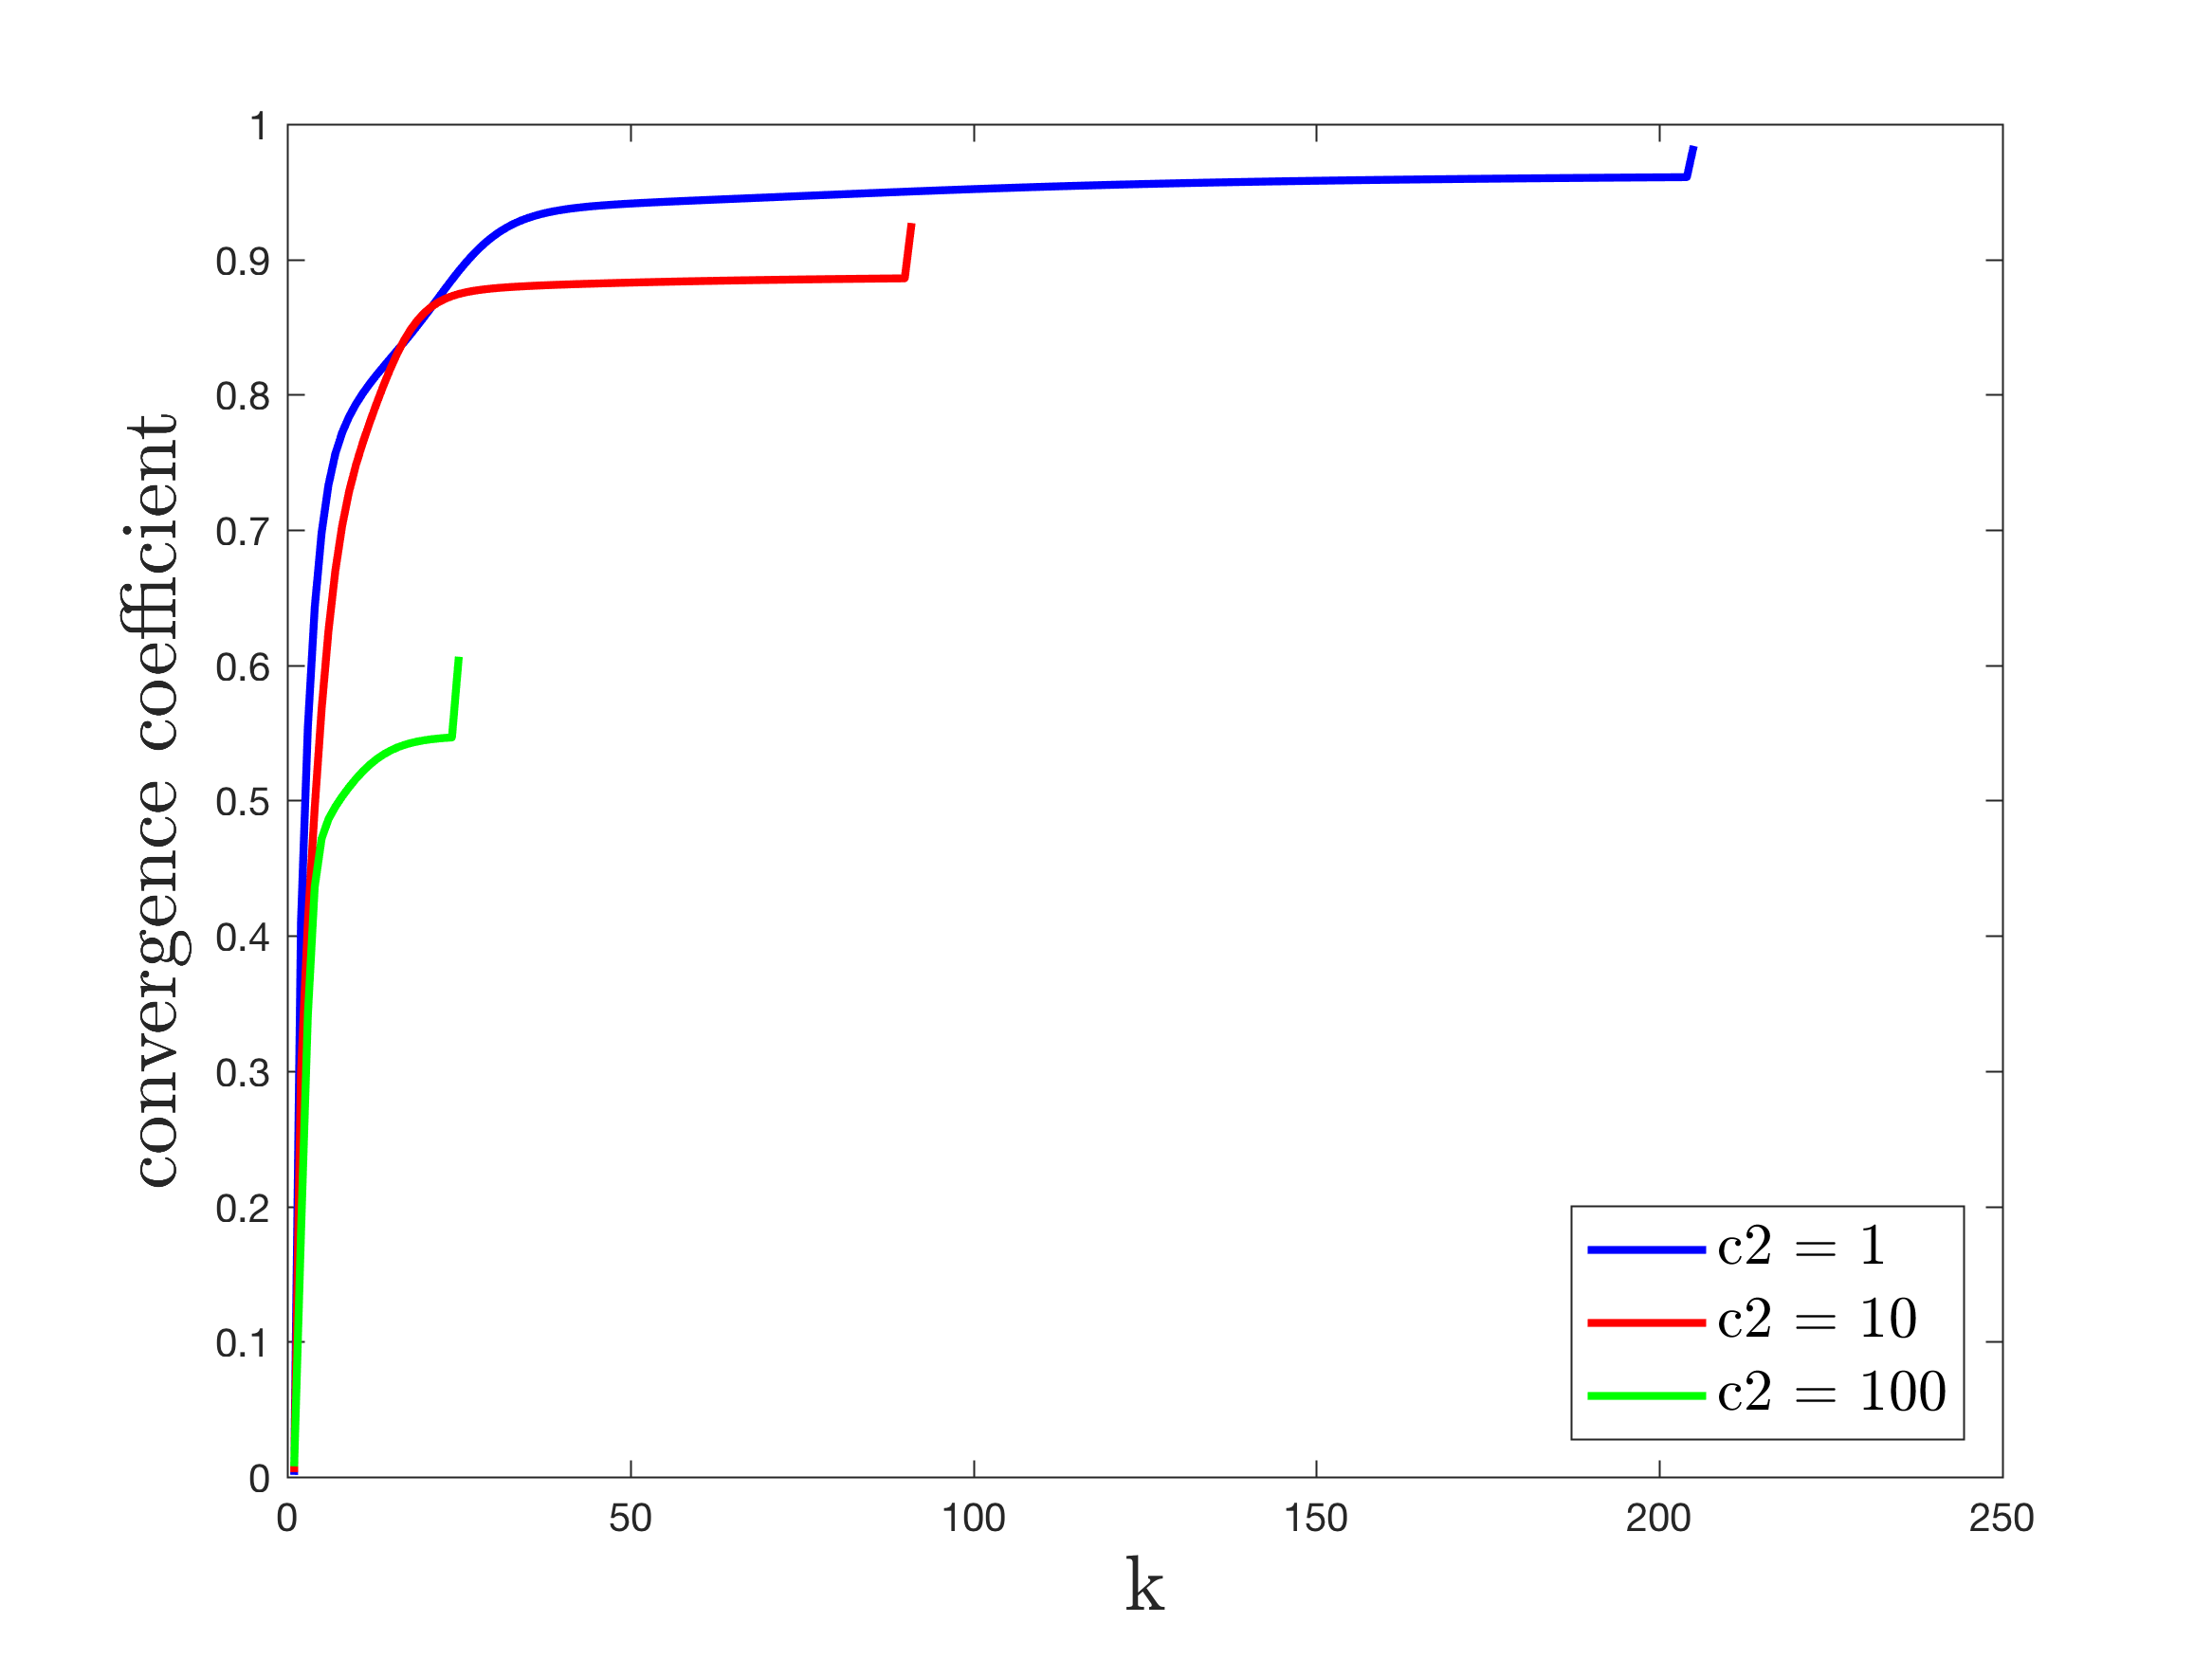
\includegraphics[scale=0.4]{images/implementation/c2_comparison/conv_rate}
	\caption{created from a fine mesh with 20 by 20 elements on a unit square, $D = 0.1$, block Jacobi smoother with block sizes of $2 \times 2$, $u_0 = max(1-2x, 0)$ and Neumann boundary conditions in time. The increase in the end may be caused by cancellation of leading digits as the  norm of the residuals for the final iterates become very small.}
\end{figure}
\textit{Question: What happens at the end there in case of convergence coefficient? Some trade off between convergence speed and accuracy? Sources? How is this solely related to eigenvalues and how much could it be other things? Also see if the smoother reacts to scaling?}

The scaling parameters in the continuous problem formulation (\ref{J_heat_equation}) do not affect the overall minimiser as we assume $J$ to be zero at the solution $[\sigma, u]$. However this is not necessarily the case in the discrete setting. The discretised problem does not necessarily have exactly zero as a minimiser. The minimiser for each of the two discrete terms may be slightly different. By changing the coefficient $c_2$ we put more emphasis on being closer to the discrete minimiser of the second term than on the first. It is however not obvious how this relates to finding the discrete solution that resembles the continuous one best. Nevertheless it slightly changes the final solution we obtain. For any fixed ratio of $c_1$ and $c_2$ we will nevertheless converge to the continuous solution by increasing the resolution of the mesh.

%\begin{table}
%	\centering
%	\begin{tabular}{|c|c|c|c|c|c|c|c|}
%		\hline
%		test case & $d$ & $c_2$& $\kappa(H)$ & $\kappa(H_{\sigma \sigma})$ & $\kappa(H_{u u})$ & smallest eigenvalue & Iter until Conv \\ \hline
%		\toprule
%		2& 0.1&1& 4707& 584 &  1786& & 205 \\ \hline
%		5& 1&1& 1505 & 584 & 1416 & &313 \\ \hline
%		11& 0.1&10&764 & 320 & 712 & &91 \\ \hline
%		20& 0.1&100&731 & 59 &  711& &25 \\ \hline
%	\end{tabular}
%	\caption{norm difference between solutions.}
%\end{table}

%We can see that the difference between the solutions reduces as we increase the accuracy of the mesh. 

%The parameter $c_2$ appears in the following terms and which we will keep in mind for the more detailed analysis of the eigenvalues later on. 
\begin{ceqn}
	\begin{equation}
	\begin{aligned}
H_{\sigma \sigma}: c_2 \langle \phi_i, \phi_j \rangle, \quad H_{\sigma u}: c_2 \langle (\phi_i)_t, (\phi_j)_x \rangle, \quad H_{u \sigma}: c_2 \langle (\phi_j)_t, (\phi_i)_x \rangle \quad H_{uu}: c_2 \langle (\phi_i)_x, (\phi_j)_x \rangle
	\end{aligned}
	\end{equation}
\end{ceqn}

The diffusion constant also has a major effect on the speed of convergence. However in contrast to the paramter $c_2$ it also changes the overall continuous solution. And the influence it was is not that straight forward to see. Therefore we will now focus our attention on an analysis of the eigenvalues and the condition number of the arising matrices. 
%Diffusion constant does not occur in $B_{\sigma \sigma}$, otherwise it occurs in the term following terms $- D \langle \nabla v, \tau \rangle$ in $B_{\sigma u}$ and $B_{u \sigma}$ and in $B_{u u} $ as $ D^2 \langle \nabla v, \nabla w \rangle$.

In order to do so we look at the eigenvalues in comparison for those test cases that work well and those that don't really work at all.

% do analysis of coarse grid correction
% for the particular problem one is looking 
% how to divide sections? 
% block Jacobi, write different version
% analyse difference, error doesnt seem smooth in space, but can't really see it when looking at solution ... 


We also looked at the eigenvalues and condition numbers of the Hessians for different parameters in order to better understand if this could potentially be related to the slow rate of convergence. It makes sense to consider them together as for regular symmetric matrices we have that $\kappa(H) = \frac{\lambda_{\text{max}}(H)}{\lambda_{\text{min}}(H)}$. The table below contains more information on the condition numbers of the Hessians and its submatrices. The numbers in the test case column correspond to those test cases from Table (\ref{table:convergence_results}). 

\begin{table}
	\centering
	\begin{tabular}{|c|c|c|c|c|c|c|c|}
		\hline
		test case & $d$ & $c_2$& $\kappa(H)$ & $\kappa(H_{\sigma \sigma})$ & $\kappa(H_{u u})$ & smallest eigenvalue & Iter until Conv \\ \hline
		\toprule
		2& 0.1&1& 4707& 584 &  1786& $8.4 \cdot 10^{-4}$ & 205 \\ \hline
		5& 1&1& 1505 & 584 & 1416 & $2.6 \cdot 10^{-3}$ &313 \\ \hline
		11& 0.1&10&764 & 320 & 712 & $5.2 \cdot 10^{-3}$ &91 \\ \hline
		20& 0.1&100&731 & 59 &  711&$5.6 \cdot 10^{-3}$ &25 \\ \hline
	\end{tabular}
	\caption{More detailed table with condition numbers. $d$ describes the diffusion constant. $c_2$ scaling parameter of the second term of the functional. $\kappa(H)$: condition number of the Hessian. $\kappa(H_{\sigma \sigma})$ : condition number of the submatrix $H_{\sigma \sigma}$, and for $H_{uu}$ respectively. All test cases are of the same size.}
	\label{table:cond_number_eig_val}
\end{table}
We can see from Table (\ref{table:cond_number_eig_val}) that there seems to be correlation between the condition number and the iterations until convergence for some cases but not for all. When we look at the condition number of the individual blocks, then $H_{\sigma \sigma}$ usually has a much smaller condition number compared to $H_{uu}$. The off-diagonal blocks are singular and therefore we cannot consider them by themselves. If we now also take the graphs below under consideration, we can see that the eigenvalues mostly vary in their small eigenvalues. But this cannot be the only factor as we can see from the fact that test case two took more iterations until convergence than test case five, even though it has a much larger condition number. Additionally we can see that test case 11 and 20 almost have the same overall condition number, but the condition number of the $H_{\sigma \sigma}$ blocks differ a lot, as well as the required iterations until convergence. 

\begin{figure}
	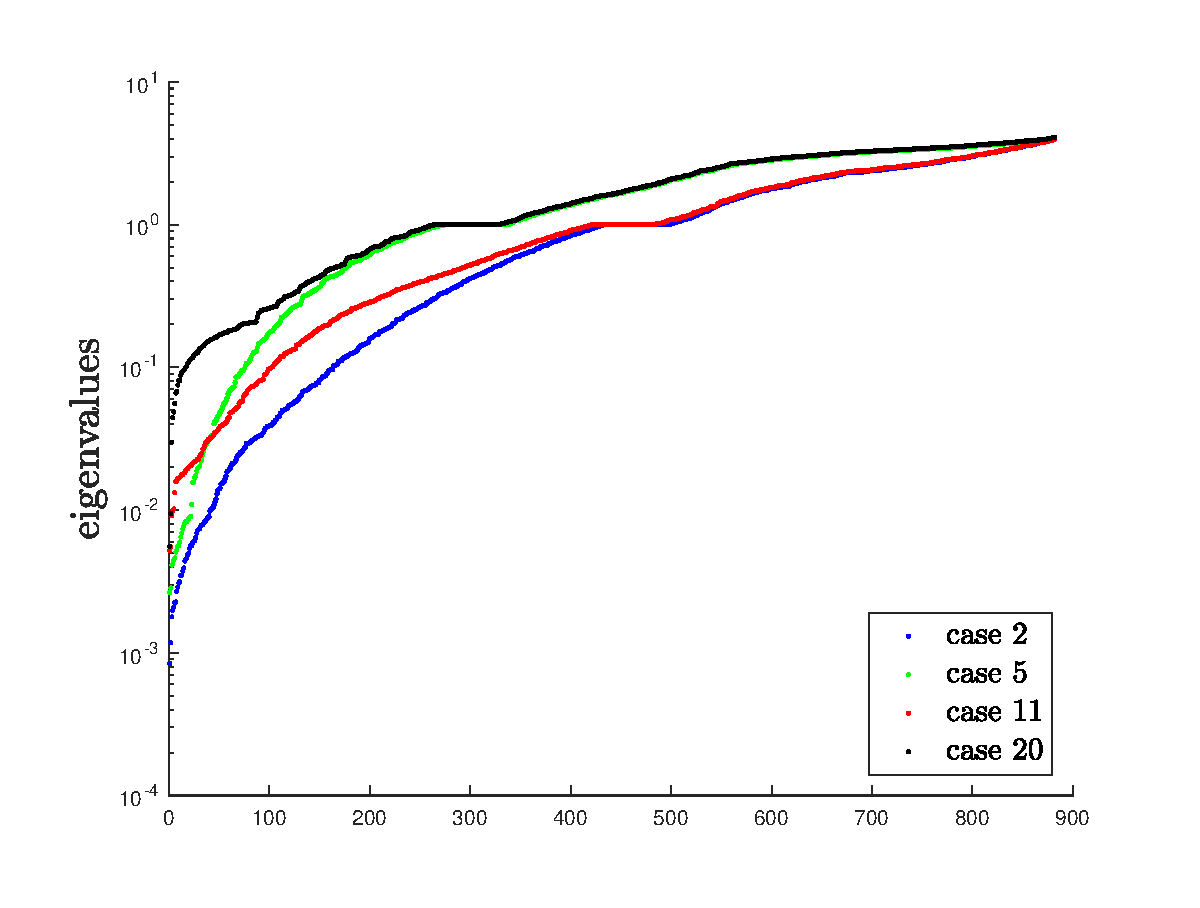
\includegraphics[scale=0.4]{images/implementation/eigenvalues/some_eigenvalues_logy}
	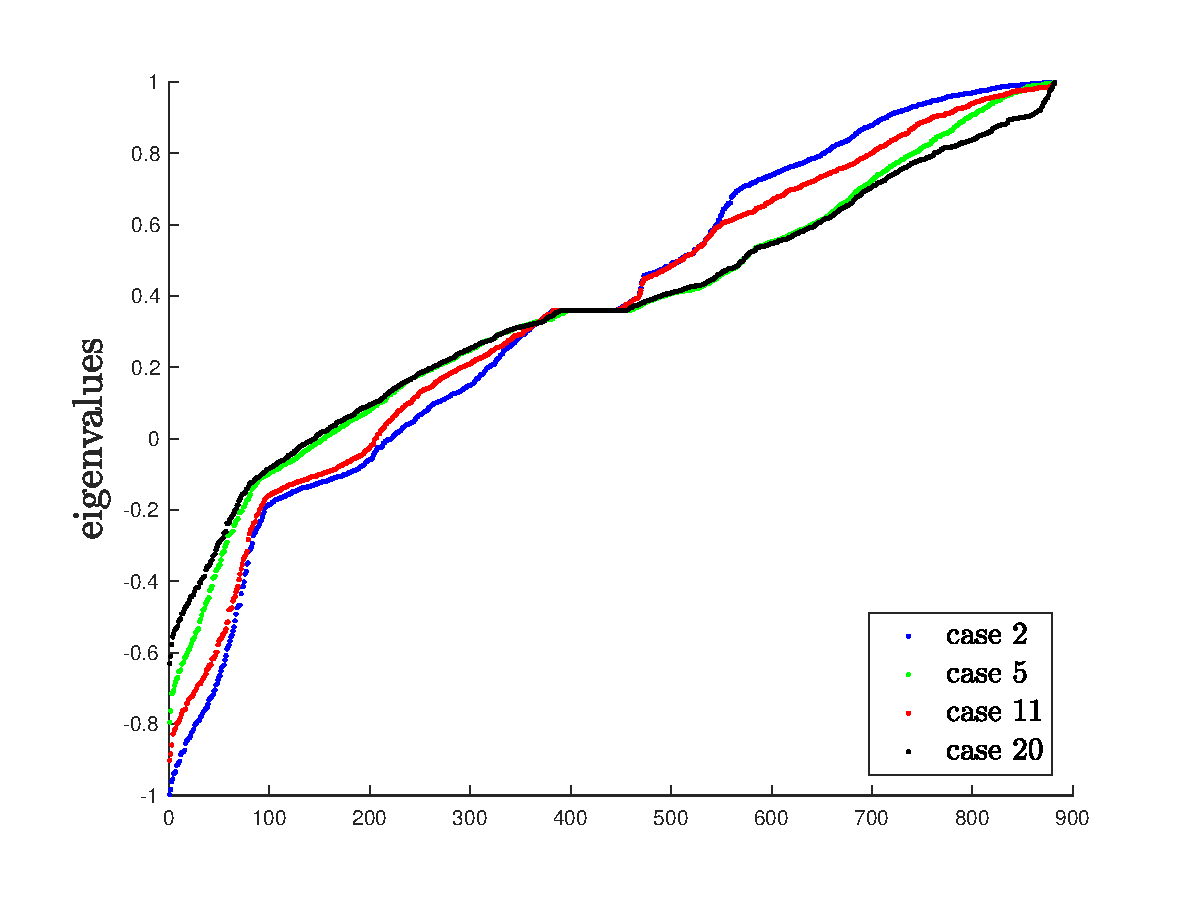
\includegraphics[scale=0.4]{images/implementation/eigenvalues/plot_eigenvalues_iter_mat_block_Jac_tc}
	\caption{Left-Panel: Sorted eigenvalues of the Hessian of the test cases $2,5,11$ and 20, using a logscale on the $y$-axis. Right-Panel: Sorted eigenvalues of the iteration matrix $M = (I - PH)$ for the same test cases, where $P$ is the preconditioner arising from the block Jacobi smoother using patches of size $2 \times 2$.}
	\label{fig:eigenvalues_H_and_it_mat}
\end{figure}

In Figure (\ref{fig:eigenvalues_H_and_it_mat}) we can see the eigenvalues of the Hessians of the same test cases as well as the eigenvalues of the iteration matrix of the relaxation scheme. We can see that the larger eigenvalues of the Hessian seem to be pretty identical in all four cases. Additionally we can say that the distribution of the eigenvalues can probably not be described by a smooth function, as in the case of the Laplacian however, they seem to be distributed fairly regularly. The plateau at one is due to the enforced boundary conditions. All of the Hessians give rise to \textit{reasonable} condition numbers, as we have seen in the table. Now we also considered the eigenvalues of the iteration matrix of the relaxation scheme using the $2 \times 2$ Jacobi block-smoother, which can be seen on the left. Due to the damping factor $\omega = 0.64$ the plateau of the imposed boundary conditions is not at zero as one would expect. If we then consider test cases 22 to 24 in comparison things look entirely different. Here the condition number seems to hardly affect the number of iterations. 
\begin{figure}
	%\includegraphics[scale=0.4]{images/implementation/eigenvalues/some_eigenvalues_logy_c2100}
	%\includegraphics[scale=0.4]{images/implementation/eigenvalues/plot_eigenvalues_iter_mat_block_Jac_tc_c2100}
	\caption{Left-Panel: Sorted eigenvalues of the Hessian of the test cases $22, 23$ and 24, using a logscale on the $y$-axis. Right-Panel: Sorted eigenvalues of the iteration matrix $M = (I - PH)$ for the same test cases, where $P$ is the preconditioner arising from the block Jacobi smoother using patches of size $2 \times 2$.}
	\label{fig:eigenvalues_H_and_it_mat}
\end{figure}

%In comparison the eigenvalues of the one-dimensional Laplace equation describe a sine function [source]. We even have that the condition number here is higher. 

%\begin{figure}[h!]
%	\centering
%	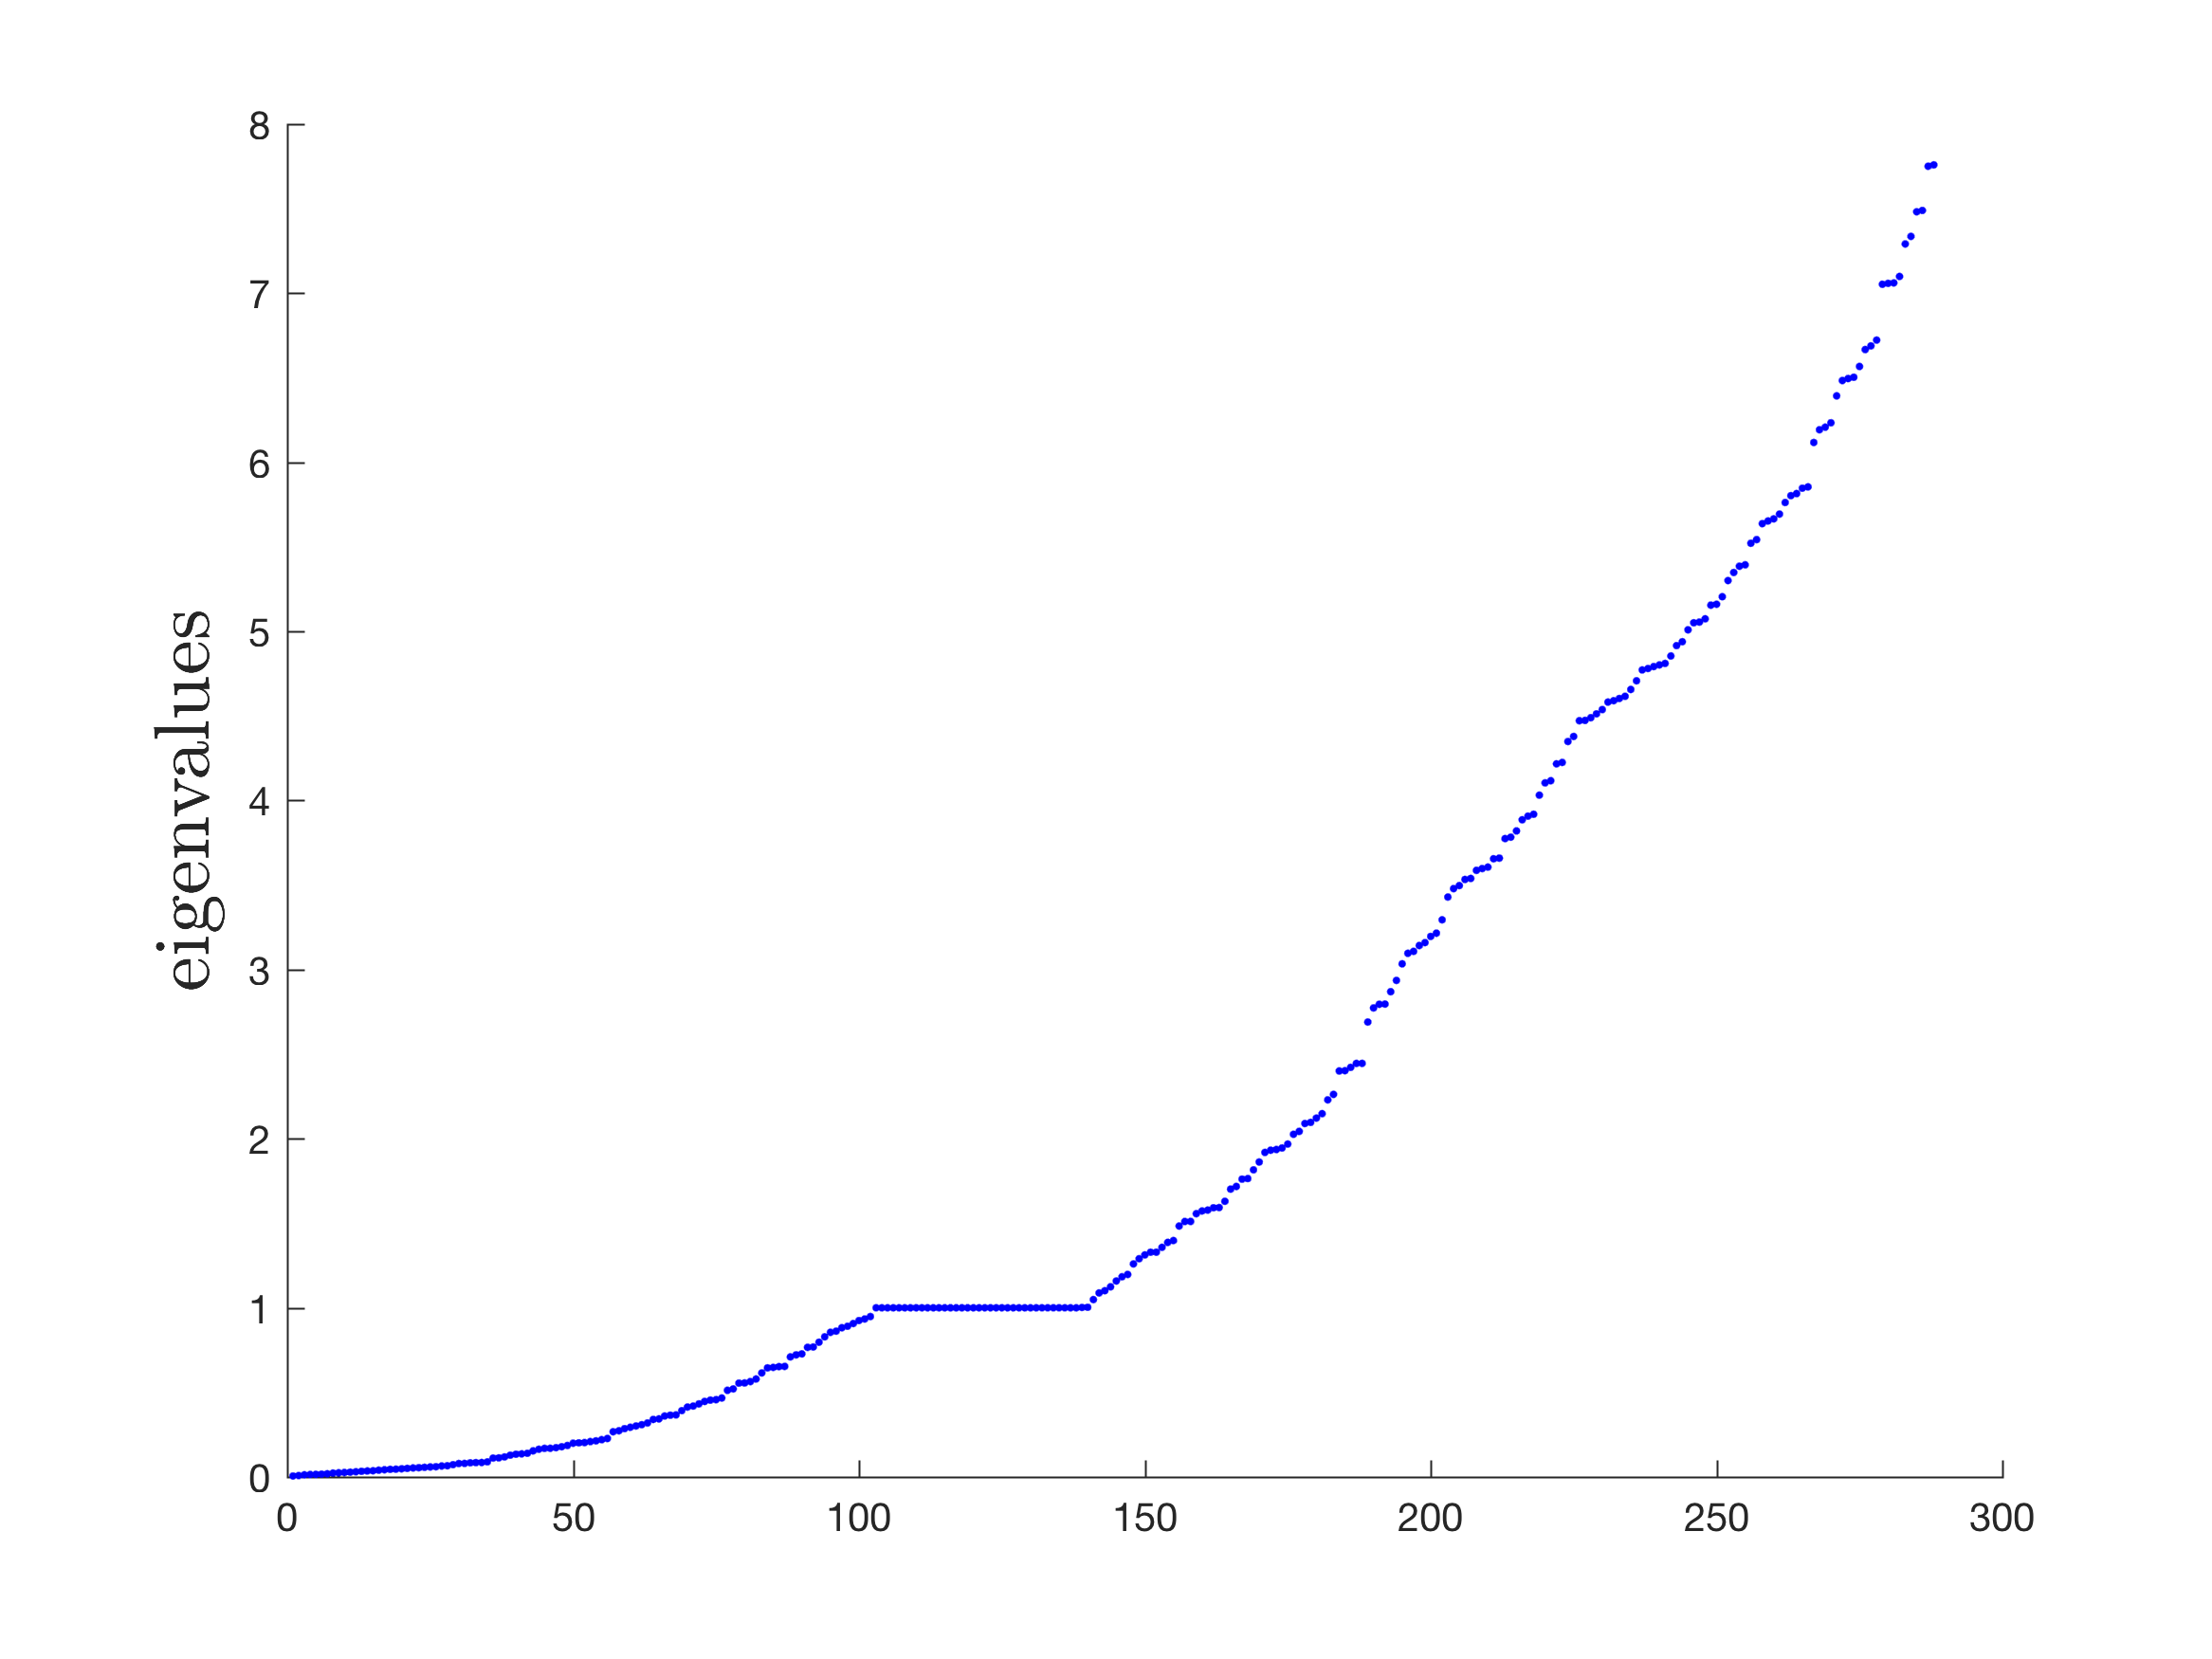
\includegraphics[scale=0.4]{images/implementation/eigenvalues/eigenvalues_11by11elem}
%	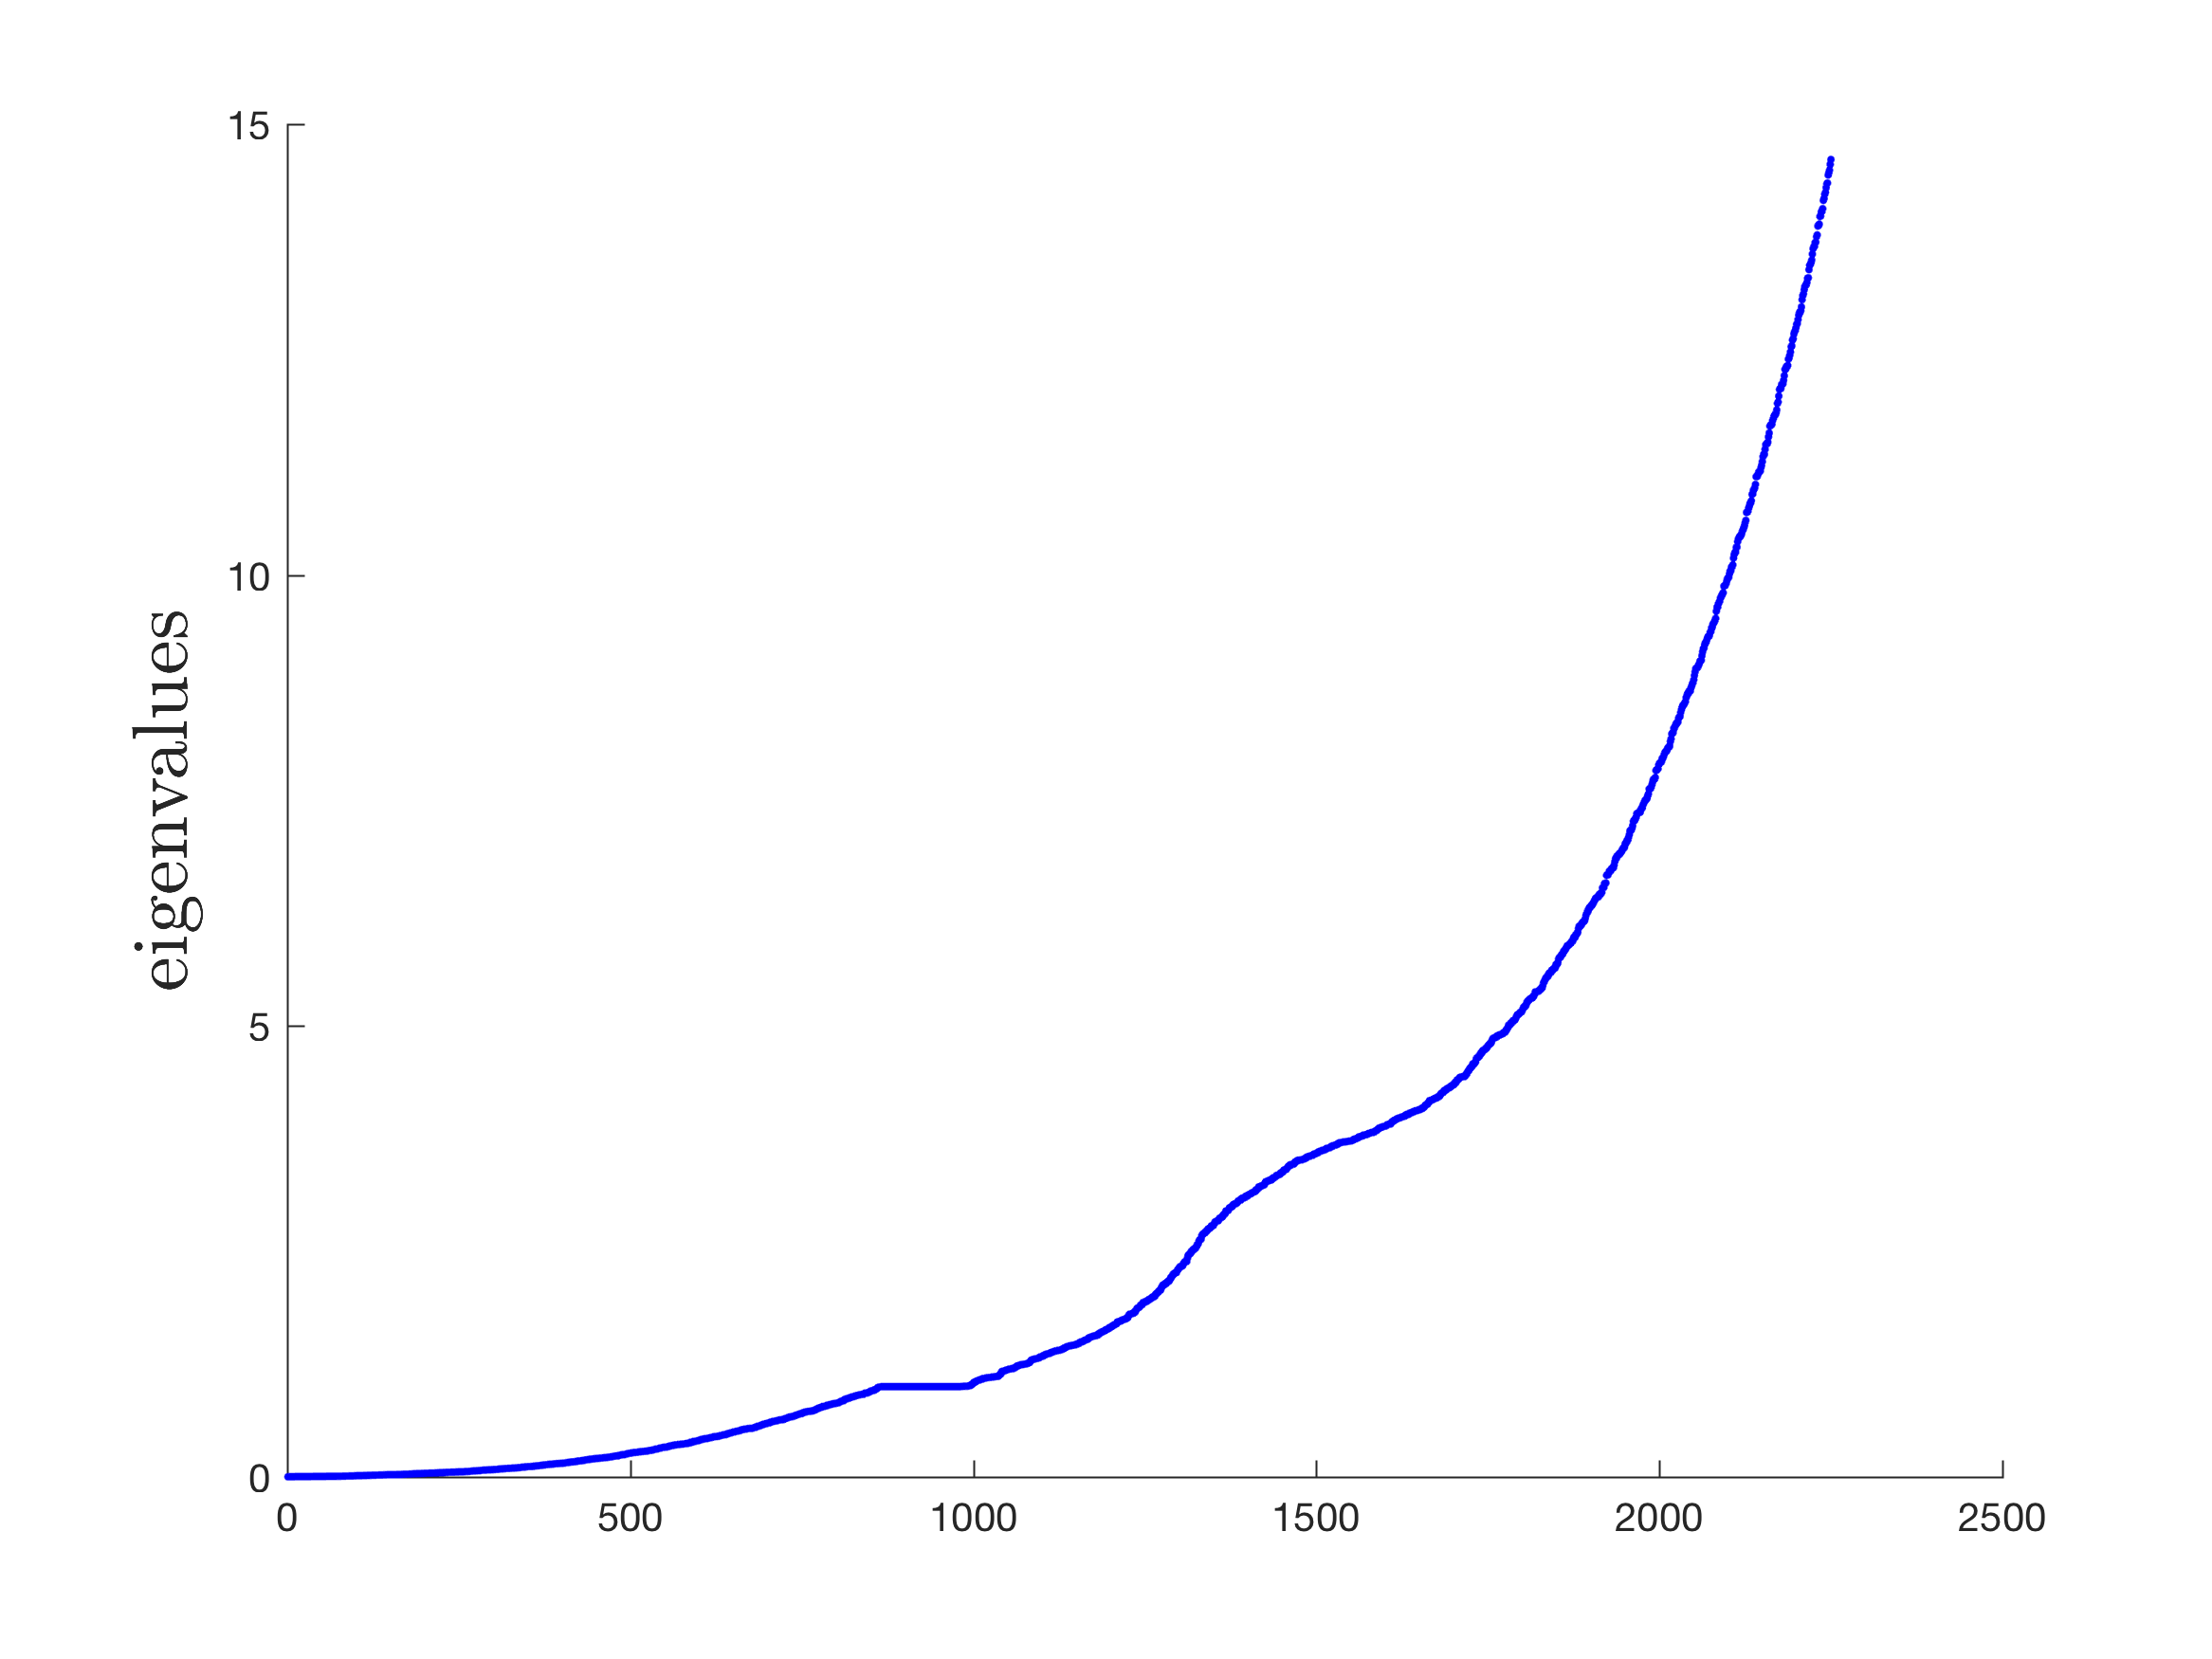
\includegraphics[scale=0.4]{images/implementation/eigenvalues/eigenvalues_24by44elem}
%	\caption{Left--Panel: Sorted eigenvalues of the Hessian $H$ using 11 elements in both space and time with $\kappa(H)=1.5\cdot10^3$. Right--Panel:   Sorted eigenvalues of the Hessian using 24 in space and 44 in time  with $\kappa(H)=23\cdot10^3$. In both cases $\Omega = (0,1)^2$.}
%\end{figure}


%\textit{next step would be to look at how these are damped? Or which ones remain? Where else could the problem be? Some eigenmodes just not damped. What was that Helmholtz thing?}

%We can see that the eigenvalues of the iteration matrix above seem to be reasonable distributed. If we consider the error in an eigenvector basis, that is if 

%\begin{ceqn}
%	\begin{equation}
%	\begin{aligned}
%	\end{aligned}
%	\end{equation}
%\end{ceqn}

We also tested the algorithm using different initial iterates for $\sigma$ and $u$. In the cases shown above we initially set $\sigma(x_k, t_l) = 0$ for all $(k, l)$ and $u(\cdot, t_l) = u_0$ for all $l$. However this did not seem to have a big effect on the convergence speed as we also tested for other initial iterates which all lead to very similar or the same number of iterations until convergence. This is in line with the above results in the sense that the first iterations the residual reduction happens quite quickly and then slows down a lot. 
 \smallskip
 \\
 We additionally compared the usage of either a coarse grid operator constructed by a Galerkin projection through the interpolation and restriction as well as a direct assembly of the Hessian on the coarse grid. They performed similarly although the Galerkin assembly tends to lead to a slighlty better convergence rate. This is probably due to the fact that it represents the actual projection of the fine grid problem and not a separate related problem.
 \smallskip
 \\
 From the analysis done so far it is yet not very clear where exactly the slow rate of convergence stems from. We have seen in Figure (\ref{fig:scaling_mg}) that the multigrid algorithm actually reduces the norm of the residual in every iteration. The interpolation operator we apply also seems to be working correctly, see Figure (\ref{fig:interpolation_op}). We have also tested the behavior of the smoother as well as the distribution of their eigenvalues. The smoother is displaying a notable smoothing property, see Figures (\ref{fig:smoother_1by1}) and (\ref{fig:smoother_3by4}). The eigenvalues of the arising iteration matrix seems \textit{normally} distributed. However it seems that depending on certain parameters some error modes are not reduced efficiently. We can remark that a larger parameter $c_2$ improved the performance for all test cases. The dependency on the other parameters we tested is not as straight forward. We will be discussing possibilities what this might be related to and how to overcome these problems in Chapter 7. 

\FloatBarrier
\subsection{Monodomain Equation}

After having looked at some linear test cases for the multigrid algorithm we will now examine the behavior of a nonlinear space--time least--squares finite element discretisation for the test case of a simplified monodomain equation. A simplified monodomain equation that shows the movement of an excitation front through space--time looks as follows

\begin{ceqn}
	\begin{equation}
	\begin{aligned}
	\label{my_monodomain}
	\partial_t u - div(d \nabla u) &= u (1 - u ) (u - u_{\text{thres}}), &\quad \text{ in } (0, S) \times (0,T),\\
	u(x, 0) &= u_0(x) &\text{ on } (0,S), \\
	\nabla u \cdot n &= 0 \qquad &\text{ on } (0, T) \text{ for } x \in \{0,S\},
	\end{aligned}
	\end{equation}
\end{ceqn}
for $d > 0$, and  $0 < u_{\text{thres}}  < 1$. We can see that the right-hand side is clearly nonlinear as it describes a third order polynomial. It can be shown that the equation has 3 fixed points, two stable fixed in zero and one, and an unstable fixed point in $u_{\text{thres}}$ \cite{deuflhard2011adaptive}. Hence depending on the initial conditions $u_0$ the solution will tend to either zero or one, unless it is exactly equal to the value of the unstable fixed point $u_{\text{thres}}$. If there is values larger than $u_{\text{thres}}$ that tend to one, we can observe that through the diffusive term this leads to an activation of the surrounding areas in space over time. The value of the diffusion constant $d$ governs the \textit{speed} diffusive reaction. This behavior can also be seen below in the graphs showing approximations of the solution. As mentioned before we can see that the above equation (\ref{my_monodomain}) only captures the excitation phase and not the depolarisation. The excitation of the tissue is the crucial part of the process and neglecting the depolaristion simplifies the model. 
\begin{figure}[ht!]
	\centering
	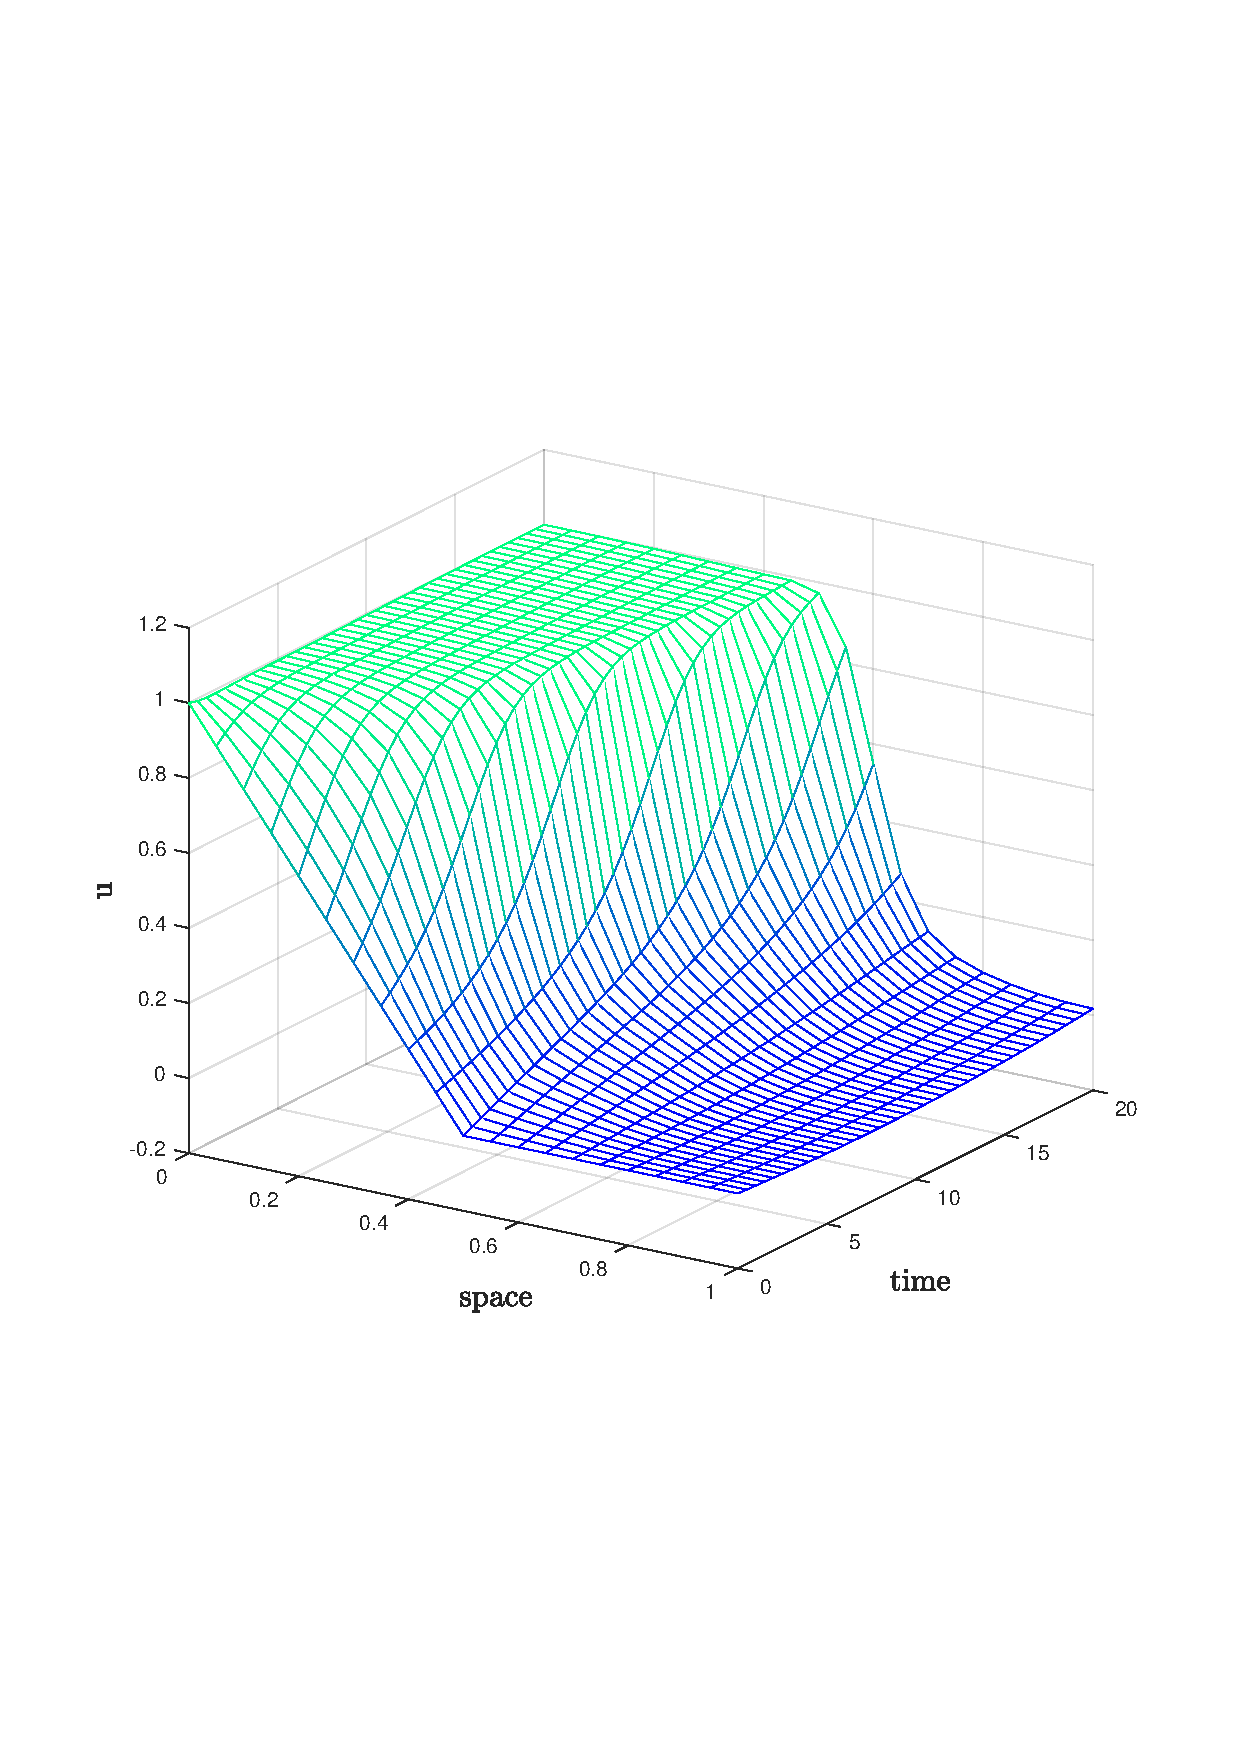
\includegraphics[scale=0.4]{images/implementation/sol_d0_001_1by20_20by40elem}
	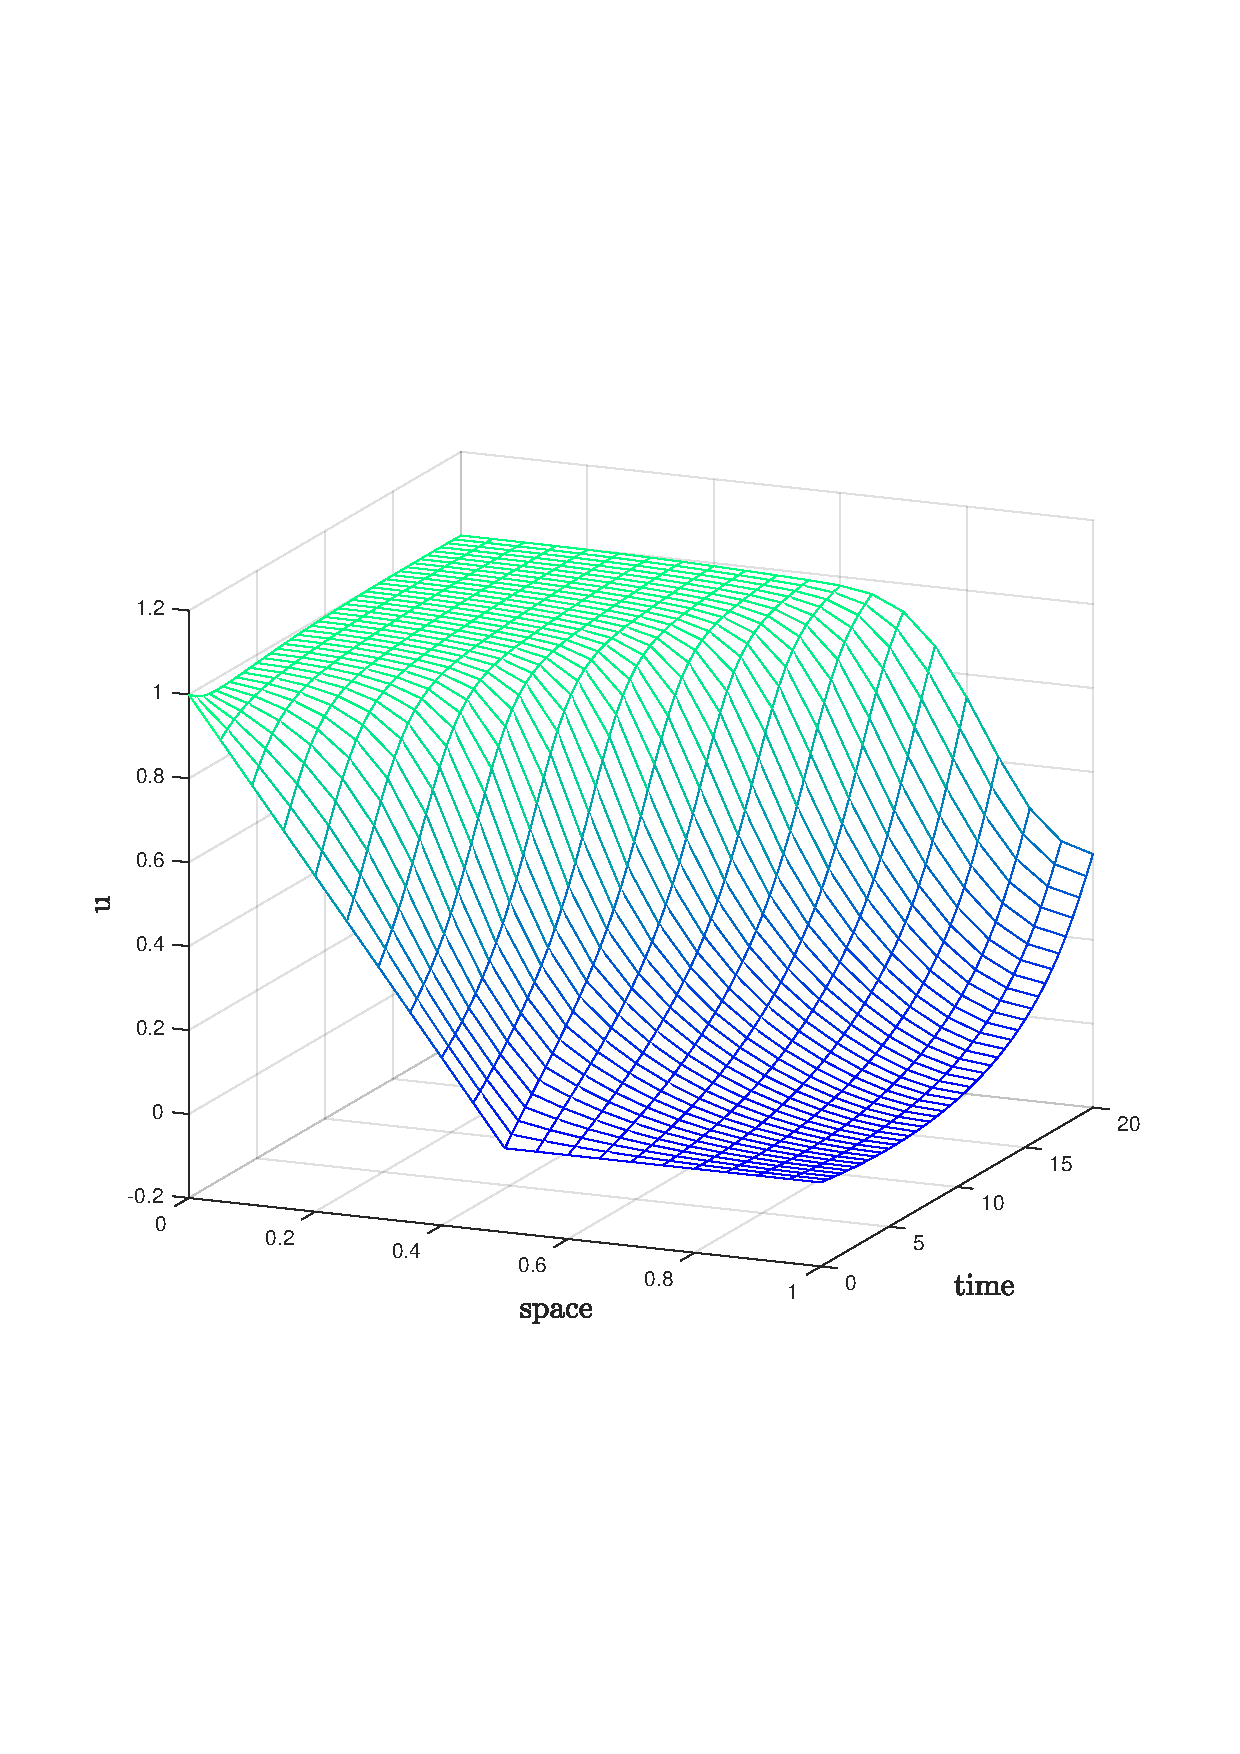
\includegraphics[scale=0.4]{images/implementation/sol_d0_003_1by20_20by40elem}
	\caption{For both graphs we have $u_0 = \max(1-2x, 0)$, homogeneous Neumann boundary conditions on the spatial boundaries of the domain, for 20 elements in space and 40 in time. Left-Panel: diffusion constant $d= 10^{-3}$. Right-Panel: $d=3 \cdot 10^{-3}$.}
	\label{fig:md_sol}
\end{figure}
The two equations giving rise to the transmembrane potentials in Figure (\ref{fig:md_sol}) only differ in the choice of the diffusion constant $d$. As to be expected we can see that with a larger value of $d$, the activation happens much more quickly. We can also see that the front is not as steep, as the electric potential spreads much faster in space.
\smallskip
\\
As previously mentioned the solutions are obtained using a dogleg trust region method, which is a combination of a gradient descent and a Newton iteration. When only using a Newton method there are iteration steps where we run into locally non-convex areas and therefore take iteration steps towards local maxima. Through the usage of a trust region method, where the algorithm first checks efficacy of the potential next step we have not experienced the same problem, but instead for each iterate obtained local convexity. 

%\textit{describe dogleg} \\
%We are using a quadratic model to approximate the functional $J$, that is we solve

%\begin{ceqn}
%	\begin{equation}
%	\begin{aligned}
%	\min_p m(p) = f + g^T p + \frac{1}{2} p^T H p \qquad s.t. \ ||p|| \leq \Delta, \ p \in \text{span}\{g, H^{-1}g\}. 
%	\end{aligned}
%	\end{equation}
%\end{ceqn}

%\begin{ceqn}
%	\begin{equation}
%	\begin{aligned}
%	p^U = - \frac{g^Tg}{g^T H g} g
%	\end{aligned}
%	\end{equation}
%\end{ceqn}

%\begin{ceqn}
%	\begin{equation}
%	\begin{aligned}
%	\tilde{p}(\tau) = \begin{cases}
%	\tau p^U \qquad &0 \leq \tau \leq 1 \\
%	p^U + (\tau - 1)(p^B - p^U) \qquad &1 \leq \tau \leq 2
%	\end{cases}
%	\end{aligned}
%	\end{equation}
%\end{ceqn}

In the dogleg algorithm there is a variety of threshold parameters that need to be chosen, and could potentially be chosen to give better convergence results, here we have restricted ourselves to some that have shown themselves to perform well on previous problem [source] (\textit{list of parameters will follow}) and not done an extensive amount of parameter tuning, as the overall aim was to develop a working nonlinear solver for now, but there are definitely many \textit{opportunities} for further testing to improve the overall performance, which we will discuss in more details in the following chapter. \\
The discretisation of the least squares formulation uses the same approximation spaces and basis as introduced in the previous sections. The nonlinear part is computed as described in section 4.5 and 4.6. 
\\
Below we can see two tables for the last iteration steps of the trust region method before reaching the convergence criterion. The parameters correspond to those depicted above in Figure (\ref{fig:md_sol}). We can see that in a neighbourhood of the respective solutions, the quadratic model seems to be a good fit to the solution, as $\rho$ is close to 1, which leads to a continually increasing trust region radius. We can also see that norm of the residual, that is $\nabla J$ decreases quickly, as one would expect when approaching the minimum of a convex neighbourhood. The tables also contain the number of accepted iterations, that is each iterations where an update actually took place, as well as the number of attempted iterations, this way one can get an insight into how often the model was determined to not be a good fit and the trust region radius was reduced without performing an update on the solution. 
\begin{table}[h!]
	\begin{center}
		\begin{tabular}{c | c | c | c | c  | c } 
			\toprule
			Accepted Iter & Overall Iter & $ || J || $ & $|| \nabla J ||$ & $\rho$ &TR Radius  \\
			\toprule
			111 & 152 & $7.520771 \cdot 10^{-5}$  & $2.3748 \cdot 10^{-4}$ & 0.835 & 192 \\ 
		%	\hline
			112 & 153 & $7.520542 \cdot 10^{-5}$ & $2.3489 \cdot 10^{-6}$ & 1.0189 & 384 \\
		%	\hline
			113 & 154 & $7.520539 \cdot 10^{-5}$ & $1.2572 \cdot 10^{-6}$ & 1.0053 & 768\\
		%	\hline
			114 & 155 & $7.520539 \cdot 10^{-5}$ & $7.1719 \cdot 10^{-11}$ & 0.9991 & 1536 \\
			\bottomrule
		\end{tabular}
	\end{center}
	\caption{Last steps of the Iteration, where $\mathcal{S} = (0, 1), \mathcal{T} = (0, 20)$, 20 elements in space, 40 elements in time, diffusion constant $d=1 \cdot 10^{-3}$, $u_{\text{init}} (\cdot,t)= u_0$ for all time steps, and $\sigma_{\text{init}} = 0$, boundary conditions as before.}
	\label{table: conv_results_small_dif}
\end{table} 


\begin{table}[h!]
	\begin{center}
		\begin{tabular}{c | c | c | c | c | c } 
			\toprule
			accepted Iter & overall Iter & $ \| J \|  $ & $|| \nabla J ||$ & $\rho $ & TR Radius \\ 
			\toprule
			62 & 84 & $1.50271 \cdot 10^{-4}$ & $1.9825 \cdot 10^{-5}$ &  1.029 & 96 \\ 
			%\hline
			63 & 85 & $1.50269 \cdot 10^{-4}$ & $2.653 \cdot 10^{-5}$ & 1.0002 & 192 \\
			%\hline
			64 & 86 & $1.50268 \cdot 10^{-4}$ & $6.582 \cdot 10^{-9}$ & 1.00045 & 384 \\
			%\hline
			65 & 87 & $1.50268 \cdot 10^{-4}$ & $7.061 \cdot 10^{-12}$ & 1.14 & 768 \\
			\bottomrule
			
		\end{tabular}
	\end{center}
	\caption{Last steps of the Iteration, where $\mathcal{S} = (0, 1), \mathcal{T} = (0, 20)$, 20 elements in space, 40 elements in time, diffusion constant $d=3 \cdot 10^{-3}$, $u_{\text{init}} (\cdot,t)= u_0$ for all time steps, and $\sigma_{\text{init}} = 0$, boundary conditions as before.}
		\label{table: conv_results_bigger_dif}
\end{table}


\begin{table}[h!]
	\begin{center}
		\begin{tabular}{c | c | c | c | c | c } 
			\toprule
			accepted Iter & overall Iter & $ \| J \|  $ & $|| \nabla J ||$ & $\rho $ & TR Radius \\ 
			\toprule
			62 & 84 & $1.50271 \cdot 10^{-4}$ & $1.9825 \cdot 10^{-5}$ &  1.029 & 96 \\ 
			%\hline
			63 & 85 & $1.50269 \cdot 10^{-4}$ & $2.653 \cdot 10^{-5}$ & 1.0002 & 192 \\
			%\hline
			64 & 86 & $1.50268 \cdot 10^{-4}$ & $6.582 \cdot 10^{-9}$ & 1.00045 & 384 \\
			%\hline
			65 & 87 & $1.50268 \cdot 10^{-4}$ & $7.061 \cdot 10^{-12}$ & 1.14 & 768 \\
			\bottomrule
			
		\end{tabular}
	\end{center}
	\caption{Testing the effect of the diffusion constant $d$ on the number of iterations until stopping criterion is met. $\mathcal{S} = (0, 1)$,  $\mathcal{T} = (0, 20)$, 20 elements in space, 40 elements in time, $u_{\text{init}} (\cdot,t)= u_0$ for all time steps, and $\sigma_{\text{init}} = 0$, boundary conditions as before.}
\end{table}

As before the two problems differ only in the diffusion constant. We can see that with a higher diffusion constant the problem converges faster. In order to see how the diffusion term affects the complexity of the problem, tested it for more parameters. 

We saw in Figure (\ref{fig:md_sol}) that with an increasing diffusion constant the overall solution has less steep gradients. more One could suppose that  \textit{Problem becomes more elliptic?!}.
\\


We also tested how the resolution affected the number of energy minimisation steps needed to reach the stopping criterion. 
\begin{table}[h!]
	\begin{center}
		\begin{tabular}{c | c | c | c | c | c | c} 
			\toprule
			space int & $N_x$ & time int & $N_t$ & accepted Iter & overall Iter & $\| \nabla J \|$ \\ 
			\toprule
			$(0,1)$ & 20 & $(0,10 )$ & 40 & 41 & 74 & \\ 
			%\hline
			$(0,1)$ & 20 & $(0,20 )$ & 40 & 65 & 87 & \\ 
			%\hline
			$(0,1)$ & 20 & $(0,20 )$ & 80 & 84 & 148 & \\ 
			%\hline
			$(0,1)$ & 40 & $(0,20 )$ & 80 & 57 & 92 & \\ 
			%\hline
			$(0,2)$ & 40 & $(0,20 )$ & 80 & 73 & 101 & \\
			%\hline
			%$(0,2)$ & 40 & $(0,40)$ & 200 & 73 & 101 & \\  
			\bottomrule
			
		\end{tabular}
	\end{center}
	\caption{different resolution and different domain sizes, diffusion constant $d=3 \cdot 10^{-3}$, $u_{\text{init}} (\cdot,t)= u_0$ for all time steps, and $\sigma_{\text{init}} = 0$. With the same boundary conditions as before. Stopping criterion $ \| \nabla J \| < 10^{-9}$}
	\label{table:diff_grids_md}
\end{table}

.
% However as we can see this criterion was not always met. What happened instead is that the algorithm \textit{got stuck there}, reducing the trust region radius more and more. While the coefficient $\rho$ grew immensely, as we can see in the table below. 




%\textit{what does this mean?}
%however by visually checking the solution we seem to obtain the correct result. Therefore what might this be?  

We can conlcude that the arising energy minimisation problem from the discretised monodomain equation has a rather complicated non-convex solution landscape. As we increase the impact of the diffusive term it converges faster which one could suppose implies that the problem becomes "more elliptic"? \textit{Can I say that? And what else should I say here?}

\FloatBarrier
\subsection{Linearisation of a Monodomain Equation}

After considering the full nonlinear problem we particularly draw our attention to its linearisation in a neighbourhood of the solution $s$. Our aim is for one to better understand the properties governing the behavior of the solution. And secondly to have a closer look at how the multigrid algorithm performs in this case, to see if we behavior we have seen in  the previous section on the heat equation repeats itself here. Or if due to the additional linearised forcing term we observe different dynamics. Under the assumption that we have a unique local minimiser of the problem, we know that we have convexity close to the solution, that is the Hessian $H_s = H(s)$ is positive definite and the gradient is very close to zero. From the previous section we know that this really is the case, see Table (\ref{table: conv_results_small_dif}) and Table (\ref{table: conv_results_bigger_dif}). 

%For small diffusion constants it previously did not seem to perform so well. In the case of the simplified monodomain equation they were even smaller than before as this is closer to realistic simulations. 


% \begin{ceqn}
%	\begin{equation}
%	\begin{aligned}
%	u_{k+1} &= u_k - H_k^{-1}(\nabla J_k) \\
%	H_k u_{k+1} &= H_k u_k - \nabla J_k, \\ 
%	\text{ let } r_k &:= H_k u_k - \nabla J_k
%	\end{aligned}
%	\end{equation}
%\end{ceqn}
%	\text{ and solve } H_k u_{k+1} = r_k \quad \text{using multigrid}

\textit{picture, residual convergence MULTIGRID to follow }
\smallskip
\\

Additionally in order to better understand the behavior of the Hessian around the solution we perform an error analysis using a Jacobi smoother on the linearised system. More specifically we want to see how small pertubations in the solution in areas of the wavefront and the constant regions behave under the iteration of the smoother. One of the intentions behind this idea was to potentially construct adapted coarse level spaces that take these different local behaviors into account. We expect the pertubations on the wavefront to be damped much slower than on the areas that have converged to the two stable fixed points. We therfore consider the following iteration 
\begin{ceqn}
	\begin{equation}
	\begin{aligned}
e_{k+1} &= e_k + P(\nabla J - H_s e_k) \quad \text{ or} \\
e_{k+1} &= e_k - P H_s e_k 
	\end{aligned}
	\end{equation}
\end{ceqn}
if we assume exactly that $\nabla J = 0$, and where $P$ describes the preconditioner. We now let $e_0$ equal to zero except for a small pertubation either in the area of the wavefront or the constant regions and see how this behaves under iteration.


\begin{figure}[ht!]
	\centering
	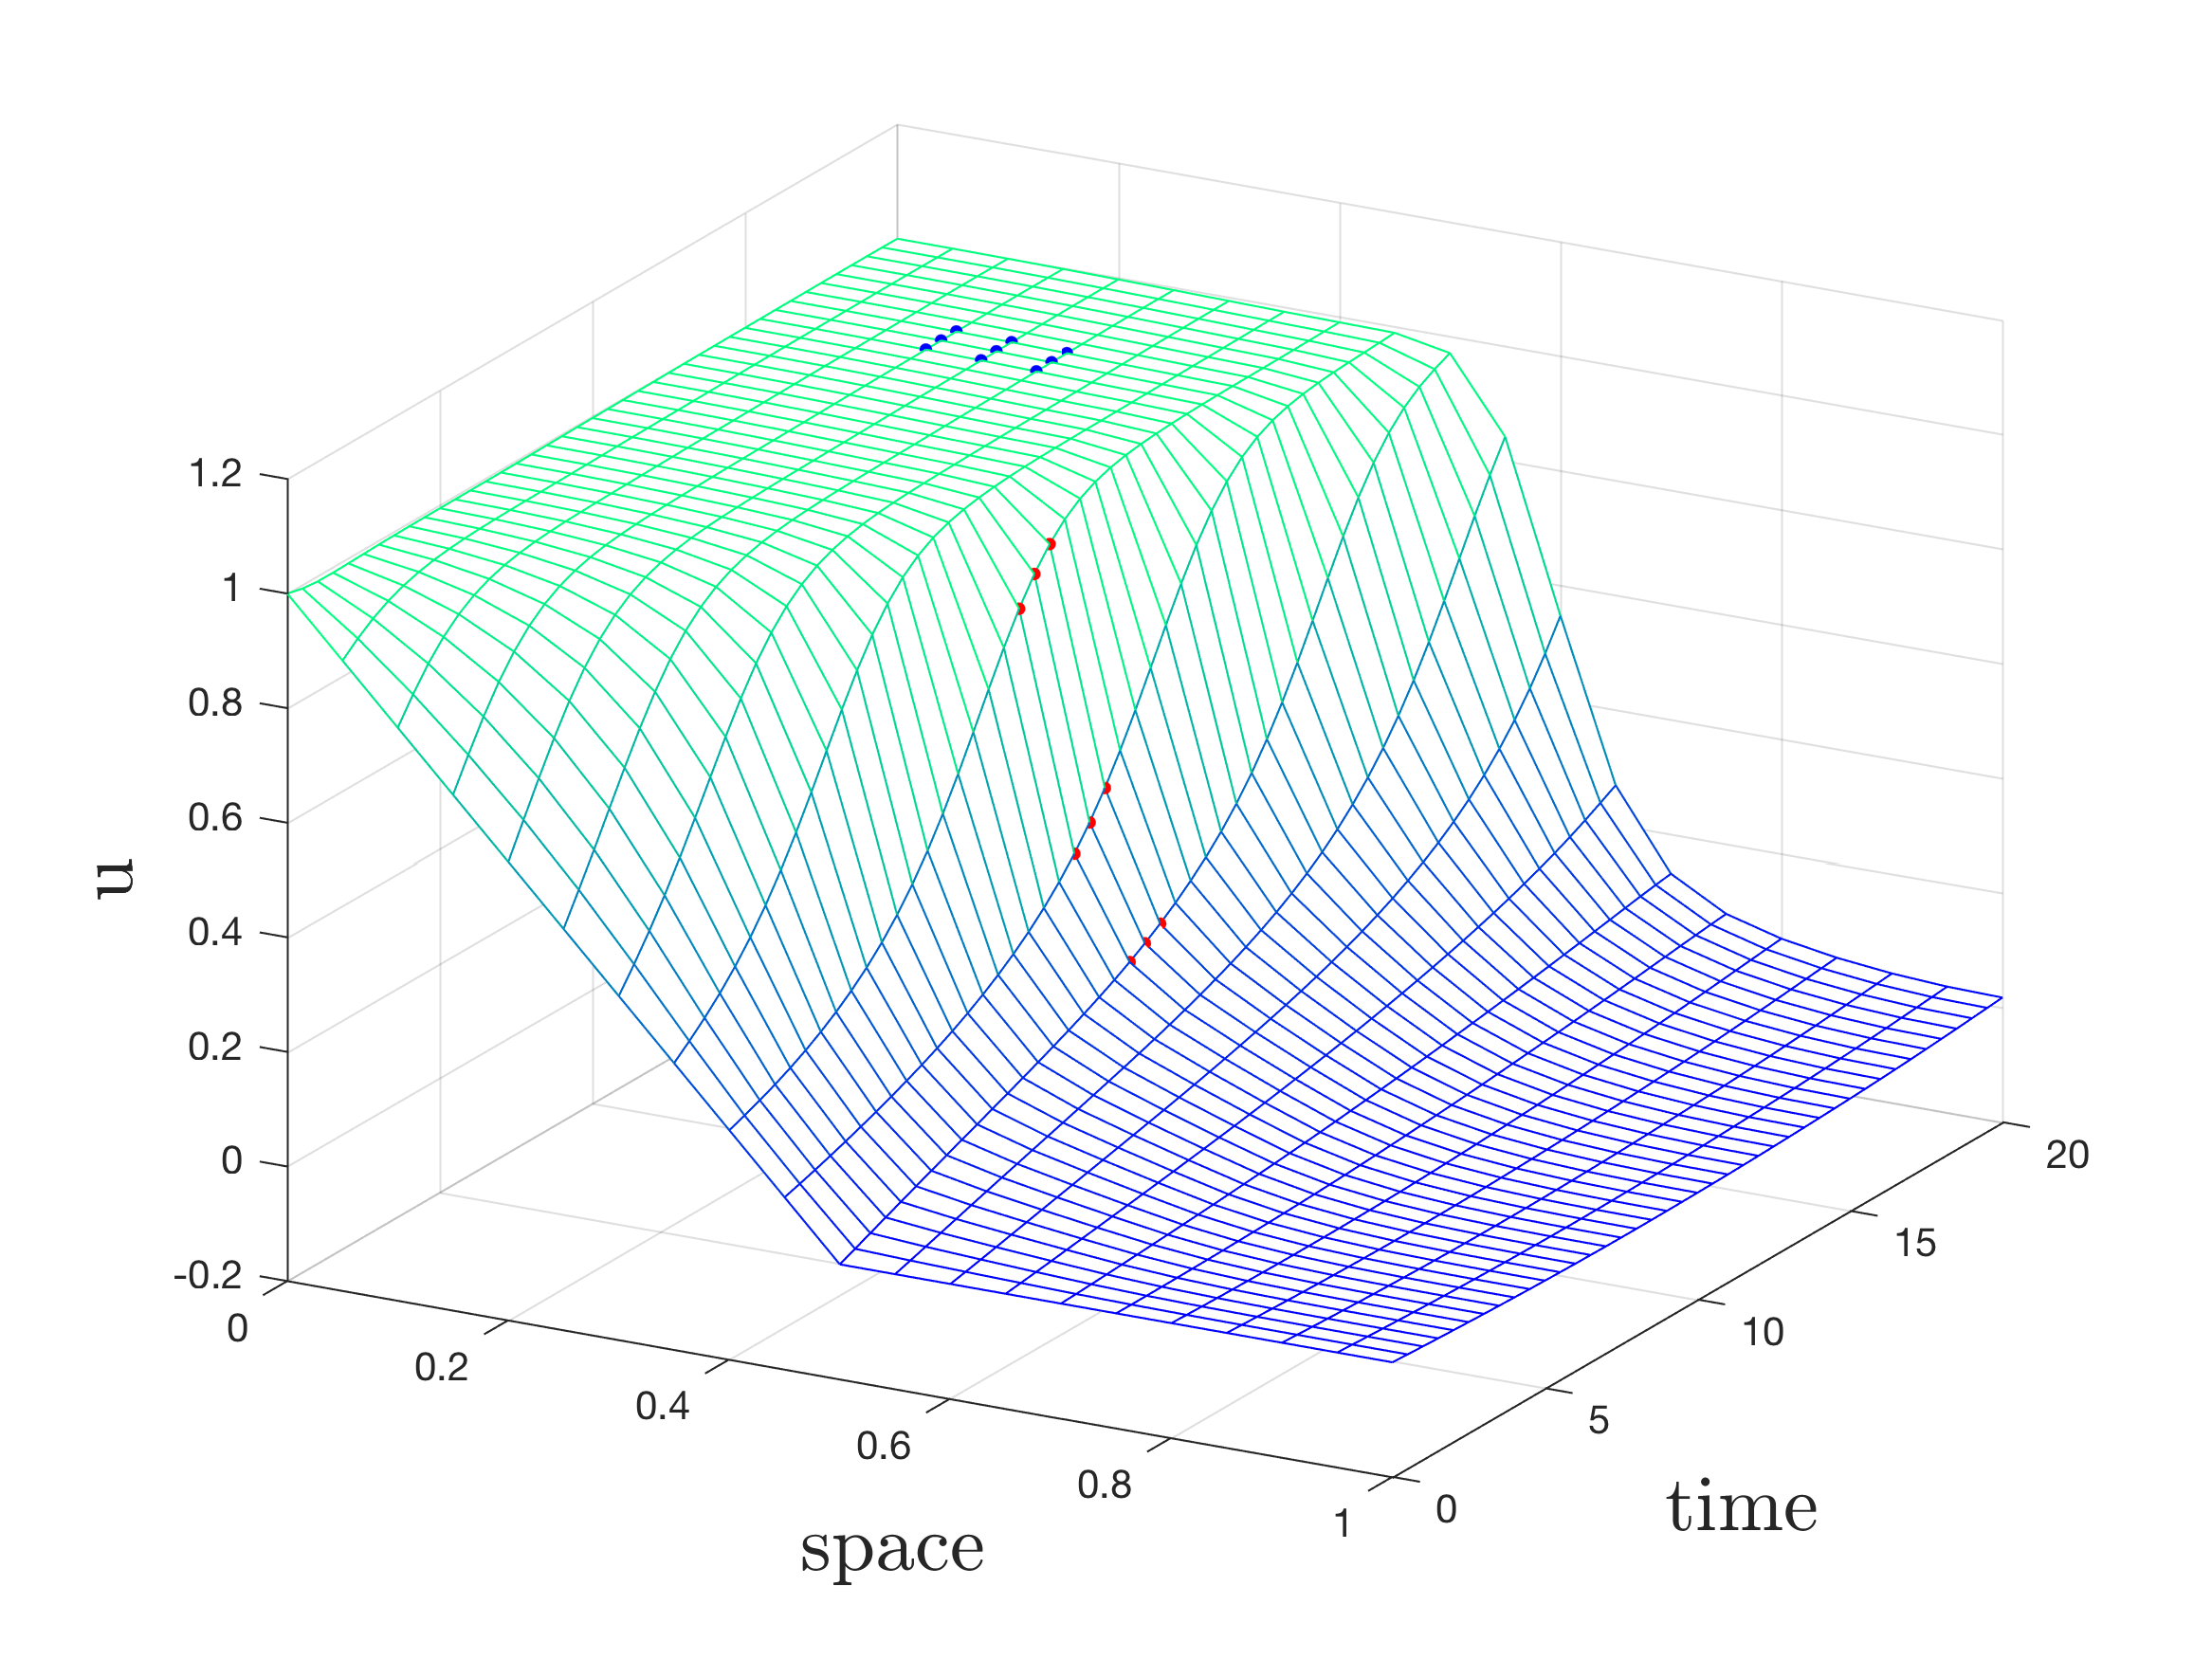
\includegraphics[scale=0.4]{images/implementation/lin_hessian/subsets_on_sol}
	\includegraphics[scale=0.4]{images/implementation/lin_hessian/res_norm}
	\caption{On the left, subsets of grid points on the constant zone, using solution for $d=1 \cdot 10^{-3}$, and on the wavefront where we set the pertubations. On the right the residual norms after each iteration for one of the random test sets.}
	\label{fig:pertubations}
\end{figure}

On average the residual norm of the perturbed areas decrease by the following contraction factors

\begin{ceqn}
	\begin{equation}
	\begin{aligned}
|| e_k^{const} || \leq 0.075 \cdot 0.756^k, \qquad || e_k^{wf} || \leq 0.068 \cdot 0.801^k, \quad 0 \leq k \leq 10
	\end{aligned}
	\end{equation}
\end{ceqn}

where $k$ describes the number of iterations, $e^{const}$ the perturbed vector on the constant area and $e^{wf}$ on the wavefront, with random pertubations between $0$ and $0.1$ on the marked areas respectively. The numbers were computed averaging over a sample test set of size $100$. We can see that pertubations on the wavefront are damped slower, which we can also see in figure \ref{fig:pertubations}, however this effect is not as drastic. Further experiments for differently sized patches and on different areas of the domain were conducted which lead to similar results.
\\
 \textit{So what to take from this, how to write this up better?}







%As with most other numerical approximations there is a great number of paramters that could be tuned, choices that could have been made differently, which will be discussed in the following chapter.

\end{document}